\documentclass[11pt,ngerman]{scrartcl}

% standard packages
\usepackage[utf8]{inputenc}  % input in UTF-8
\usepackage[T1]{fontenc}  % output in T1 fonts (westeuropäische Codierung)
\usepackage{lmodern}  % latin modern fonts
\usepackage[ngerman]{babel}  % deutsches Sprachpaket, neue Rechtschreibung

% Seitensetup
\usepackage{scrlayer-scrpage}  % Seitenformatierung durch KOMA-interne Optionen
\usepackage[top=4cm, bottom=4cm]{geometry}  % Seitengeometrie (kann durch KOMA ersetzt werden, hab ich aber nicht geschafft)
\usepackage[hypcap=false]{caption, subcaption}  % caption editing - hypcap warning with hyperref
\usepackage{array}  % table editing

% additional packages
\usepackage{amsmath, amssymb, amstext}  % math packages (American Math Society)
\usepackage{bm}
\usepackage{icomma}  % Kommata in Dezimalzahlen verursachen keinen Abstand mehr
\usepackage{graphicx}  % Bilder einfügen
\usepackage{float} %Bilder placement
\usepackage{pdfpages}  % PDF als vollständige Seiten einfügen
\usepackage{lastpage}  % referenziert die letzte Seite
\usepackage[separate-uncertainty=true]{siunitx}  % bessere Darstellung von Einheiten
\usepackage{makecell} %Dicke Tabellenstriche
\usepackage{longtable}
\usepackage{booktabs}
%\usepackage{datatool}
\usepackage[hidelinks]{hyperref}  % hyperref verlinkt Referenzen - hidelinks entfernt borders um links

% package setups
% Kopf- und Fußzeile durch KOMA
\pagestyle{scrheadings}  % KOMA darf entscheiden
\clearpairofpagestyles  % reset
\setkomafont{pageheadfoot}{\normalfont}  % Standardschrift in Kopf- und Fußzeile
\captionsetup{format=plain, font=small, labelfont=bf} %Better caption, Abbildung ist FETT
%\setlength{\headheight}{27.2pt}  % benötigte Höhe Kopfzeile (warning von scrlayer-scrpage, wird aber automatisch so gerendert, falls diese Option weggelassen wird)
\ihead{Silbercoulometer\\Elekrolyse}  % Kopf links %Todo Titel ändern
\chead{\textsc{Philipp} Maximilian \\ \textsc{Stark} Matthias}  % Kopf Mitte %Todo Name ändern
\ohead{26 November 2021}  % Kopf rechts %Todo Datum ändern
\cfoot{\pagemark \, / \pageref{LastPage}}  % Fuß Mitte

% Table of Contents
\DeclareTOCStyleEntry{dottedtocline}{section}  % KOMA intern - Inhaltsverzeichnis mit Punkten (nur sections)

%Overbar setup
\newcommand{\overbar}[1]{\mkern 1.5mu\overline{\mkern-1.5mu#1\mkern-1.5mu}\mkern 1.5mu}
% SI
\sisetup{locale = DE}  % deutschsprachige SI-Konvention
\sisetup{quotient-mode = fraction}
\sisetup{per-mode = fraction}
\DeclareSIUnit\px{px}
\DeclareSIUnit\strich{|||}
\DeclareSIUnit\torr{Torr}

% citation
\usepackage{csquotes}
\usepackage[backend=biber]{biblatex}
\addbibresource{silber.bib} %Todo .bib befüllen zb.: mit JabRef (Empfehlung der Redaktion)

%Eigene Commands
\newcommand{\der}[2]{\frac{\mathrm{d}#1}{\mathrm{d}#2}}
\newcommand{\pder}[2]{\frac{\partial #1}{\partial #2}}

%\noindent für ges
\setlength{\parindent}{0pt}


\begin{document}
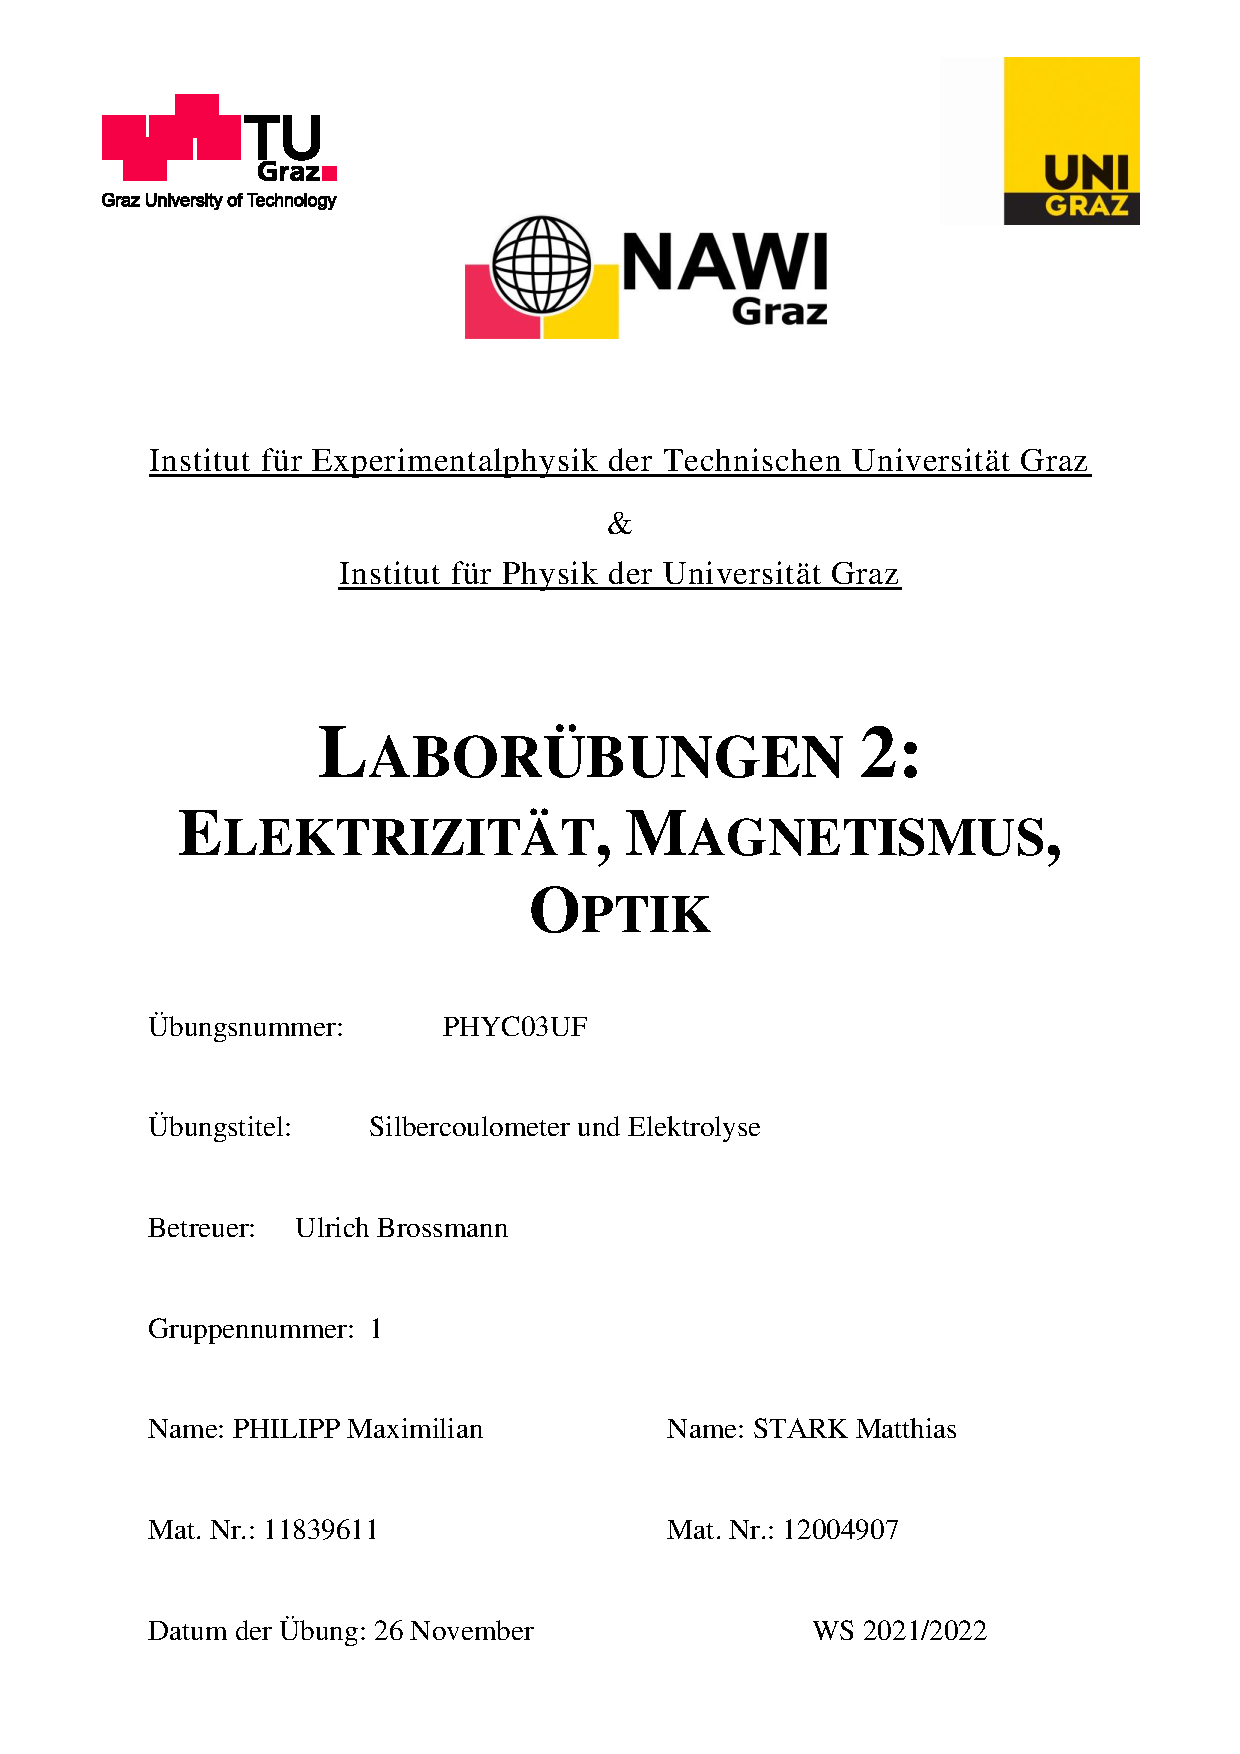
\includepdf{Deckblatt_labor2.pdf}
\tableofcontents
\newpage

\section{Aufgabenstellung\label{Auf0}}

\subsection{Silbercoulometer}

\begin{itemize}

	\item Bestimmen Sie die Faraday-Konstante mit Hilfe eines Silbercoulometers. Man wähle $I = 100$ mA, $t = 60$ min.

	\item Berechnen Sie die Größe der Elementarladung e (L = \SI{6.024 E23}{1\per\mol}).

	\item Es ist eine Fehlerabschätzung durchzuführen!

\end{itemize}


\subsection{Elektrolyse}

\begin{itemize}

	\item Es ist die Dichte der verdünnten Schwefelsäure im Hoffmann'schen Wasserzersetzungsapparat mit dem Aräometer (Senkspindel) zu bestimmen.

	\item Die durch die Elektrolyse bei verschiedenen Stromstärken und Zeitdauern (Mittelung der
	      Stromstärke über die Zeit!) entstehenden Wasserstoffmengen sind zu messen. Im speziellen
	      bei $I = 300$ mA, $t = 10$ min.

	\item Aus der abgeschiedenen Masse des Wasserstoffes soll die Faradaykonstante, das elektrochemische Äquivalent und die Größe der Elementarladung $e$ ermittelt werden.

	\item Unsicherheitsanalyse.

\end{itemize}

\newpage

\section{Grundlagen}

\subsection{Silbercoulometer}

\subsubsection{Elektrolyse und Faraday'sches Gesetz}

Die Elektrizitätsleitung in einem Elektrolyten (Lösung oder Schmelze eines heteropolaren Stoffes)
erfolgt durch Wanderung der frei beweglichen Ionen im elektrischen Feld \textbf{E} (\autoref{fig:abb1}). Ein
Ion, welches durch Aufnahme oder Abspaltung von $z$ Elektronen aus dem neutralen Atom oder
Molekül entstanden ist, nennt man $z$-wertig negativ (Anion), respektive positiv (Kation). Ein
$z$-wertiges Ion transportiert $z$ positive oder negative Elementarladungen e. An den Elektroden
werden diese abgegeben, d.h. es entsteht hier ein neutrales Teilchen, das sich entweder als solches
abscheidet oder mit dem Lösungsmittel oder mit dem Elektrodenmaterial chemisch reagiert
(Sekundärreaktion).\cite{vorlagesilber}

\begin{figure}[H]
	\begin{center}
		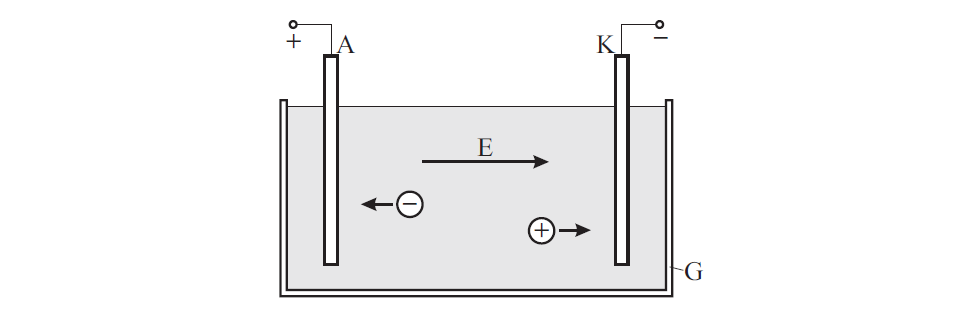
\includegraphics[width=\textwidth]{abb1}
	\end{center}
	\caption{Ionentransport im Elektrolyten im elektrischen Feld. A Anode, K Kathode}
	\label{fig:abb1}
\end{figure}


Bei jeder Elektrolyse treten also an den Elektroden chemische Vorgänge auf. Hierbei muss die
Zahl $n$ der entladenen $z$-wertigen Ionen, und damit auch die Zahl der entstehenden Atome oder
Moleküle, der durch den Elektolyten geflossenen Elektrizitätsmenge $q$ proportional sein. Es ist:

\begin{equation}
	q = n e z
\end{equation}

Wählt man für $n$ die Zahl der Moleküle pro Mol, also die Loschmidt'sche Zahl L, so ergibt sich

\begin{equation}
	Q = L e z \qquad \hat{=} \qquad \frac{Q}{z} = L e =: F = \frac{e z}{z}
\end{equation}

mit $e z$ der Ladung eines $z$-wertigen Ions.

Die Größe $Q/z = F$ ist eine von der Art des Elektrolyten unabhängige Konstante, da sie das
Produkt zweier universeller Konstanten $L$ und $e$ ist. Sie heißt Faraday-Konstante. $F$ ist nach
Gl. (2) diejenige Elektrizitätsmenge, die beim Durchgang durch einen Elektrolyten 1 Mol eines
1-wertigen oder den $z$-ten Teil eines Moles einer $z$-wertigen Ionensorte abscheidet. Die experimentelle
Bestimmung von $F$ gestattet bei bekannter Loschmidt'scher Zahl $L$ die Elektronenladung
$e$ zu berechnen oder umgekehrt.

\subsubsection{Methode zur Bestimmung von F}

Man schickt durch einen Elektrolyten während der Zeit $t$ einen genau gemessenen Strom $I$, also
eine genau bekannte Elektrizitätsmenge $q$, und bestimmt die Menge $m$ eines an einer Elektrode
abgeschiedenen Reaktionsproduktes mit dem Molekulargewicht $M$, bzw. die von einer Elektrode
abtransportierte Stoffmenge.

Ist das Ion, dessen Entstehung und Entladung zur Bildung des Stoffes führt, $z$-wertig, so ergibt
sich das Faraday'sche Gesetz

\begin{equation}
	q = I t = \frac{m}{M} F z
\end{equation}

oder:

\begin{equation}
	F = \frac{I t M}{m z}
	\label{eq:Faraday_silber}
\end{equation}

Für die Bestimmung von $F$ nach Gl. (4) wählt man Elektrolysen, die eindeutige und stabile
Reaktionsprodukte ergeben, deren Menge auf einfache Weise exakt bestimmt werden kann
(Edelmetallniederschläge). Ist $F$ bekannt, so lässt sich umgekehrt aus der Menge des transportierten
Stoffes die durch den Elektrolyten geflossene Elektrizitätsmenge ermitteln. Entsprechend
werden derartige Apparate als Coulometer bezeichnet. Hält man die Stromstärke durch ein Coulometer
zeitlich konstant, so lässt sich der Betrag von $F$ durch eine Wägung und eine Zeitmessung
sehr exakt angeben.

Wird, wie im Hoffmann'schen Zersetzungsapparat, Gas abgeschieden, muss die Masse über die
Gasgleichung bestimmt werden. Eingesetzt in Gl. (4) ergibt sich für das Experiment nach \autoref{fig:abb3}
mit $p_L$ dem Luftdruck, $p_D$ dem Dampfdruck der Lösung, $V$ dem Gasvolumen, $T$ der Gastemperatur,
$\rho$ der Dichte der Lösung, $h$ der Höhendifferenz (s. \autoref{fig:abb3}), $g$ der Erdbeschleunigung und
$R$ der allgemeinen Gaskonstanten:

\begin{equation}
	F = \frac{I t R T}{z V (p_L + \rho g h - p_D)}
	\label{eq:Faraday_elektro}
\end{equation}

Die Größe $z$ bezeichnet hier die Anzahl der pro Gasmolekül transportierten Elementarladungen.



\subsection{Elektrolyse}

Die chemische Zersetzung einer Flüssigkeit beim Durchgang eines elektrischen Stromes heißt
Elektrolyse. Derartige stromleitende Flüssigkeiten nennt man Elektrolyte. Bei diesen sind im
Gegensatz zu den Metallen (Ladungsträger sind freie Elektronen) positive und negative Ionen
Träger des elektrischen Stromes. Die Ionen entstehen beispielsweise durch Dissoziation verschiedener
Verbindungen (z.B. H$_2$SO$_4$) in Lösungsmitteln (z.B. H$_2$O). Beim Anlegen einer Spannung
an die Elektroden wandern die positiven Ionen zur Kathode (Kationen), die negativen Ionen zur
Anode (Anionen).

Ist eine Ionenart $z$-wertig, so trägt jedes ihrer Ionen die $z$-fache Elementarladung e. Werden also
$n$ Ionen abgeschieden, so geben sie insgesamt die Ladung

\begin{equation}
	Q = n z e
\end{equation}

ab. Misst man eine konstante Stromstärke $I$ über einen Zeitraum $t$, so muss die Ladung andererseits
gleich dem Produkt von $I$ und $t$ sein:

\begin{equation}
	Q = \int I dt \qquad = \qquad I t \qquad \qquad (I = \textrm{const})
\end{equation}

Hat ein Ion die Masse $m_x = m_A / N_A$, so wird insgesamt die Masse

\begin{equation}
	m = n m_x
\end{equation}

abgeschieden. $m_A$ ist die Molmasse, $m_x$ die absolute Atommasse, N$_A$ = \SI{6.02214076E23}{\per\mol} \cite{SIstandard2019} Teilchen die
Avogadro'sche oder Loschmidt'sche Zahl.

Benützt man in Gl. (8) für $n$ Gl. (6), und drückt dort $Q$ durch Gl.(7) aus, so erhält man

\begin{equation}
	m = I t \frac{m_x}{z e}
\end{equation}

Der in Gl. (9) auftretende Faktor $m_x / (ze)$ wird auch elektrochemisches Äquivalent $C$ genannt,

\begin{equation}
	C = \frac{m_x}{z e} = \frac{m_x N_A}{z e N_A} = \frac{m_A}{z F}
	\label{eq:elektrochem}
\end{equation}

woraus nach Erweiterung mit der Avogadrokonstanten $N_A$ ersichtlich ist, dass die mit $F = e N_A$
definierte Größe eine Konstante sein muss (Faradaykonstante, 1 $F$ = 96524 As/mol).
Gl. (9) enthält die Aussage des sogenannten 1. Faraday'schen Gesetzes:

\vspace{2mm}

Die an einer Elektrode abgeschiedene Stoffmenge ist der durch den Elektrolyten hindurchgegangen
Elektrizitätsmenge, d.h. dem Produkt aus Stromstärke und Zeit, proportional.

\vspace{2mm}

Ausgehend von Gl. (10) kann das 2. Faraday'sche Gesetz formuliert werden:

\vspace{2mm}

Die elektrochemischen Äquivalente zweier Stoffe verhalten sich wie ihre chemischen Äquivalente.

\vspace{2mm}

(Unter chemischem Äquivalent, Grammäquivalent oder valarer Masse versteht man die Molmasse
$m_A$, dividiert durch die Wertigkeit der Ionenart).\cite{vorlagesilber}


\newpage

\section{Versuchsanordnung}\label{sec:Versuchsanordnung}

\subsection{Silbercoulometer}

Das Ag-Coulometer ist in \autoref{fig:abb1} schematisch dargestellt. Die Anode A und die Kathode sind
aus Feinsilber Als Elektrolyt dient Silbernitrat AgNO$_3$. Silbernitrat dissoziiert in Ag$^+$ und NO$_3^-$
Die Vorgänge an den Elektroden sind:\cite{vorlagesilber}

\begin{align*}
	\textrm{Kathode}: \,\, \qquad \textrm{Ag}^+ + e \longrightarrow \textrm{Ag} \qquad \qquad \textrm{(als körniger Niederschlag)}     \\
	\,\textrm{Anode}: \qquad \quad \textrm{NO}_3^- - e \longrightarrow (\textrm{NO}_3) \qquad \qquad \textrm{(als unstabiles Radikal)} \\
	\qquad(\textrm{NO}_3) + \textrm{Ag} \longrightarrow \textrm{NO}_3^- + \textrm{Ag}^+ \qquad \qquad \qquad \qquad \qquad \quad       \\
	\\
	\textrm{Bilanz}: \qquad \quad \textrm{Ag} - e \longrightarrow \textrm{Ag}^+  \qquad \qquad \qquad \qquad \qquad \qquad \qquad \qquad
\end{align*}

Die mittlere Konzentration der AgNO$_3$ - Lösung ändert sich demnach während der Elektrolyse
nicht. Daher bleibt die Anzahl der Ladungsträger während der Messung konstant. Es ändert sich
jedoch die Beweglichkeit der Ionen durch Erwärmung des Elektrolyten. Mit steigender Temperatur
nimmt die Beweglichkeit zu, dadurch sinkt der Widerstand des Elektrolyten. Damit die
Stromstärke während der Messung konstant bleibt, muss daher die Widerstandsabnahme durch
Verringern der Spannung kompensiert werden. \autoref{fig:abb2} zeigt die Messschaltung.

\begin{figure}[H]
	\begin{center}
		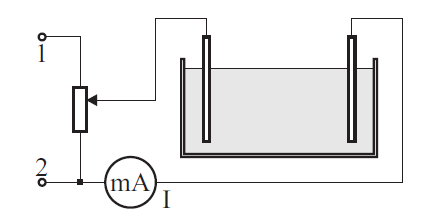
\includegraphics[width=0.6\textwidth]{abb2}
	\end{center}
	\caption{Messschaltung zur Elektrolyse. An die Punkte 1 und 2 wird eine Gleichspannung gelegt.}
	\label{fig:abb2}
\end{figure}

Das Gewicht der Elektroden ist vor Beginn und nach Beendigung der Elektrolyse im trockenen
Zustand mit einer analytischen Waage möglichst exakt zu bestimmen. Nicht sämtliche transportierte
und neutralisierte Ionen bleiben an der Kathode haften. Etliche Silberatome sinken
zu Boden (Schlammbildung). Auch in Form kleiner Kristalle abgelagertes Silber mit geringer
Haftung an der Kathode löst sich los, und geht, durch die Schwerkraft bedingt, zu Boden. Das
Gewicht der Kathode vor und nach der Elektrolyse ist daher kein genaues Maß für alle transportierten
Ionen. Da aber alle transportierten Ionen tatsächlich aus der Anode stammen, ist der
Anodengewichtsunterschied ein gutes Maß für den Materietransport.

Das Einlegen und Entfernen der Elektroden in und aus dem Elektrolyten darf nur unter Aufsicht
des Praktikumsleiters durchgeführt werden, da die AgNO$_3$ - Lösung an vielen Stoffen, vor
allem an organischen Substanzen, Zersetzungen verursacht. Auf der Haut erzeugt AgNO$_3$ - Lösung
schwarze, schwer entfernbare Flecken.

\vspace{2mm}

Der tatsächliche Aufbau ist in folgender Abbildung ersichtlich:

\begin{figure}[H]
	\begin{center}
		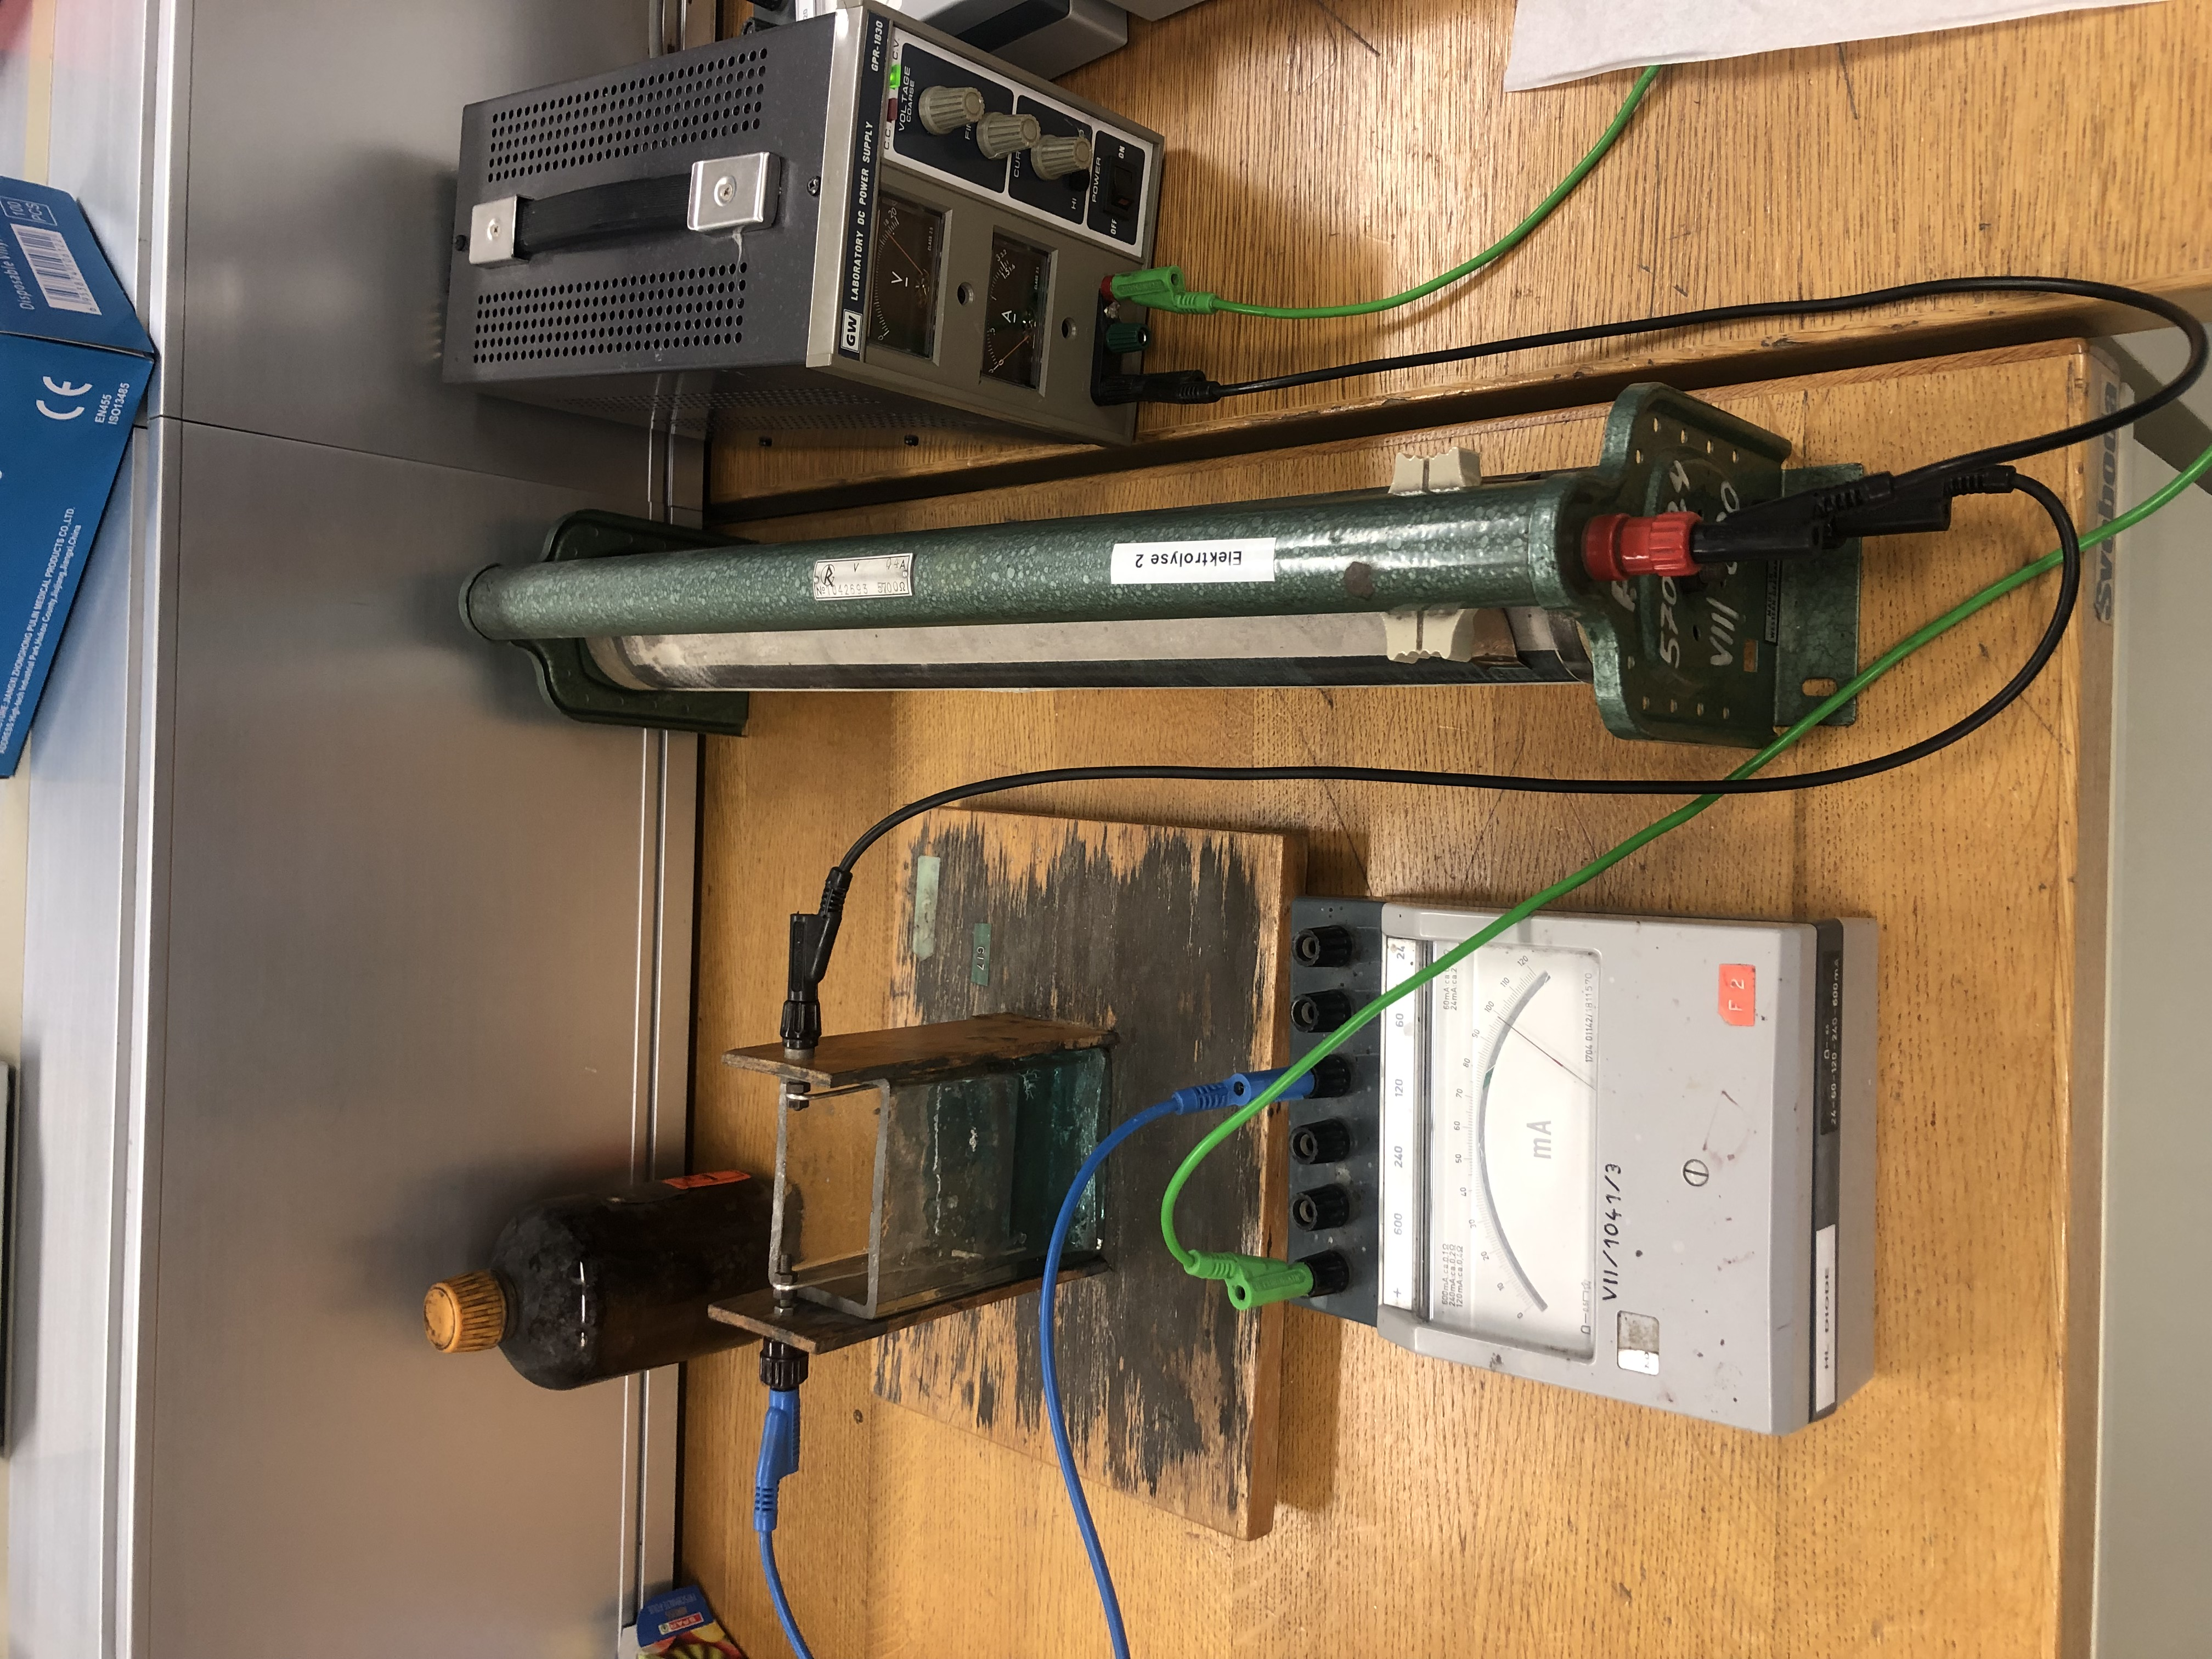
\includegraphics[angle=-90,width=0.5\textwidth]{aufbau_ag}
	\end{center}
	\caption{Versuchsaufbau des Silbercoulometers}
	\label{fig:aufbau_ag}
\end{figure}


\subsection{Elektrolyse}

Als Elektrolyt dient verdünnte Schwefelsäure. In wässriger Lösung sind positive H$^+$ - Ionen und negative SO$^{--}_4$ - Ionen vorhanden. Bei Anlegen einer Spannung nehmen die H$^+$ - Ionen an der
Kathode Elektronen auf, werden neutral und frei, den SO$^{--}_4$ - Ionen werden an der Anode negative
Ladungen entzogen. Sie setzen sich mit dem Lösungsmittel wieder zu H$_2$SO$_4$ um, wobei an der
Anode der freiwerdende Sauerstoff austritt:

\begin{equation}
	2\textrm{SO}_4 + 2\textrm{H}_2\textrm{O} = 2\textrm{H}_2\textrm{SO}_4 + \textrm{O}_2
\end{equation}

Das Experiment wird mit dem Hofmann'schen Zersetzungsapparat durchgeführt, bei dem beide
Gase getrennt aufgefangen werden können.

\begin{figure}[H]
	\begin{center}
		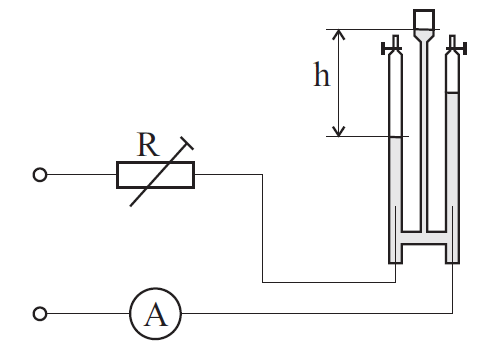
\includegraphics[width=0.5\textwidth]{abb3}
	\end{center}
	\caption{Schaltung zum Hoffmann'schen Wasserzersetzungsapparat. R bezeichnet dabei den Stellwiderstand,
		A das Amperemeter}
	\label{fig:abb3}
\end{figure}

Der tatsächliche Aufbau ist in folgender Abbildung ersichtlich:

\begin{figure}[H]
	\begin{center}
		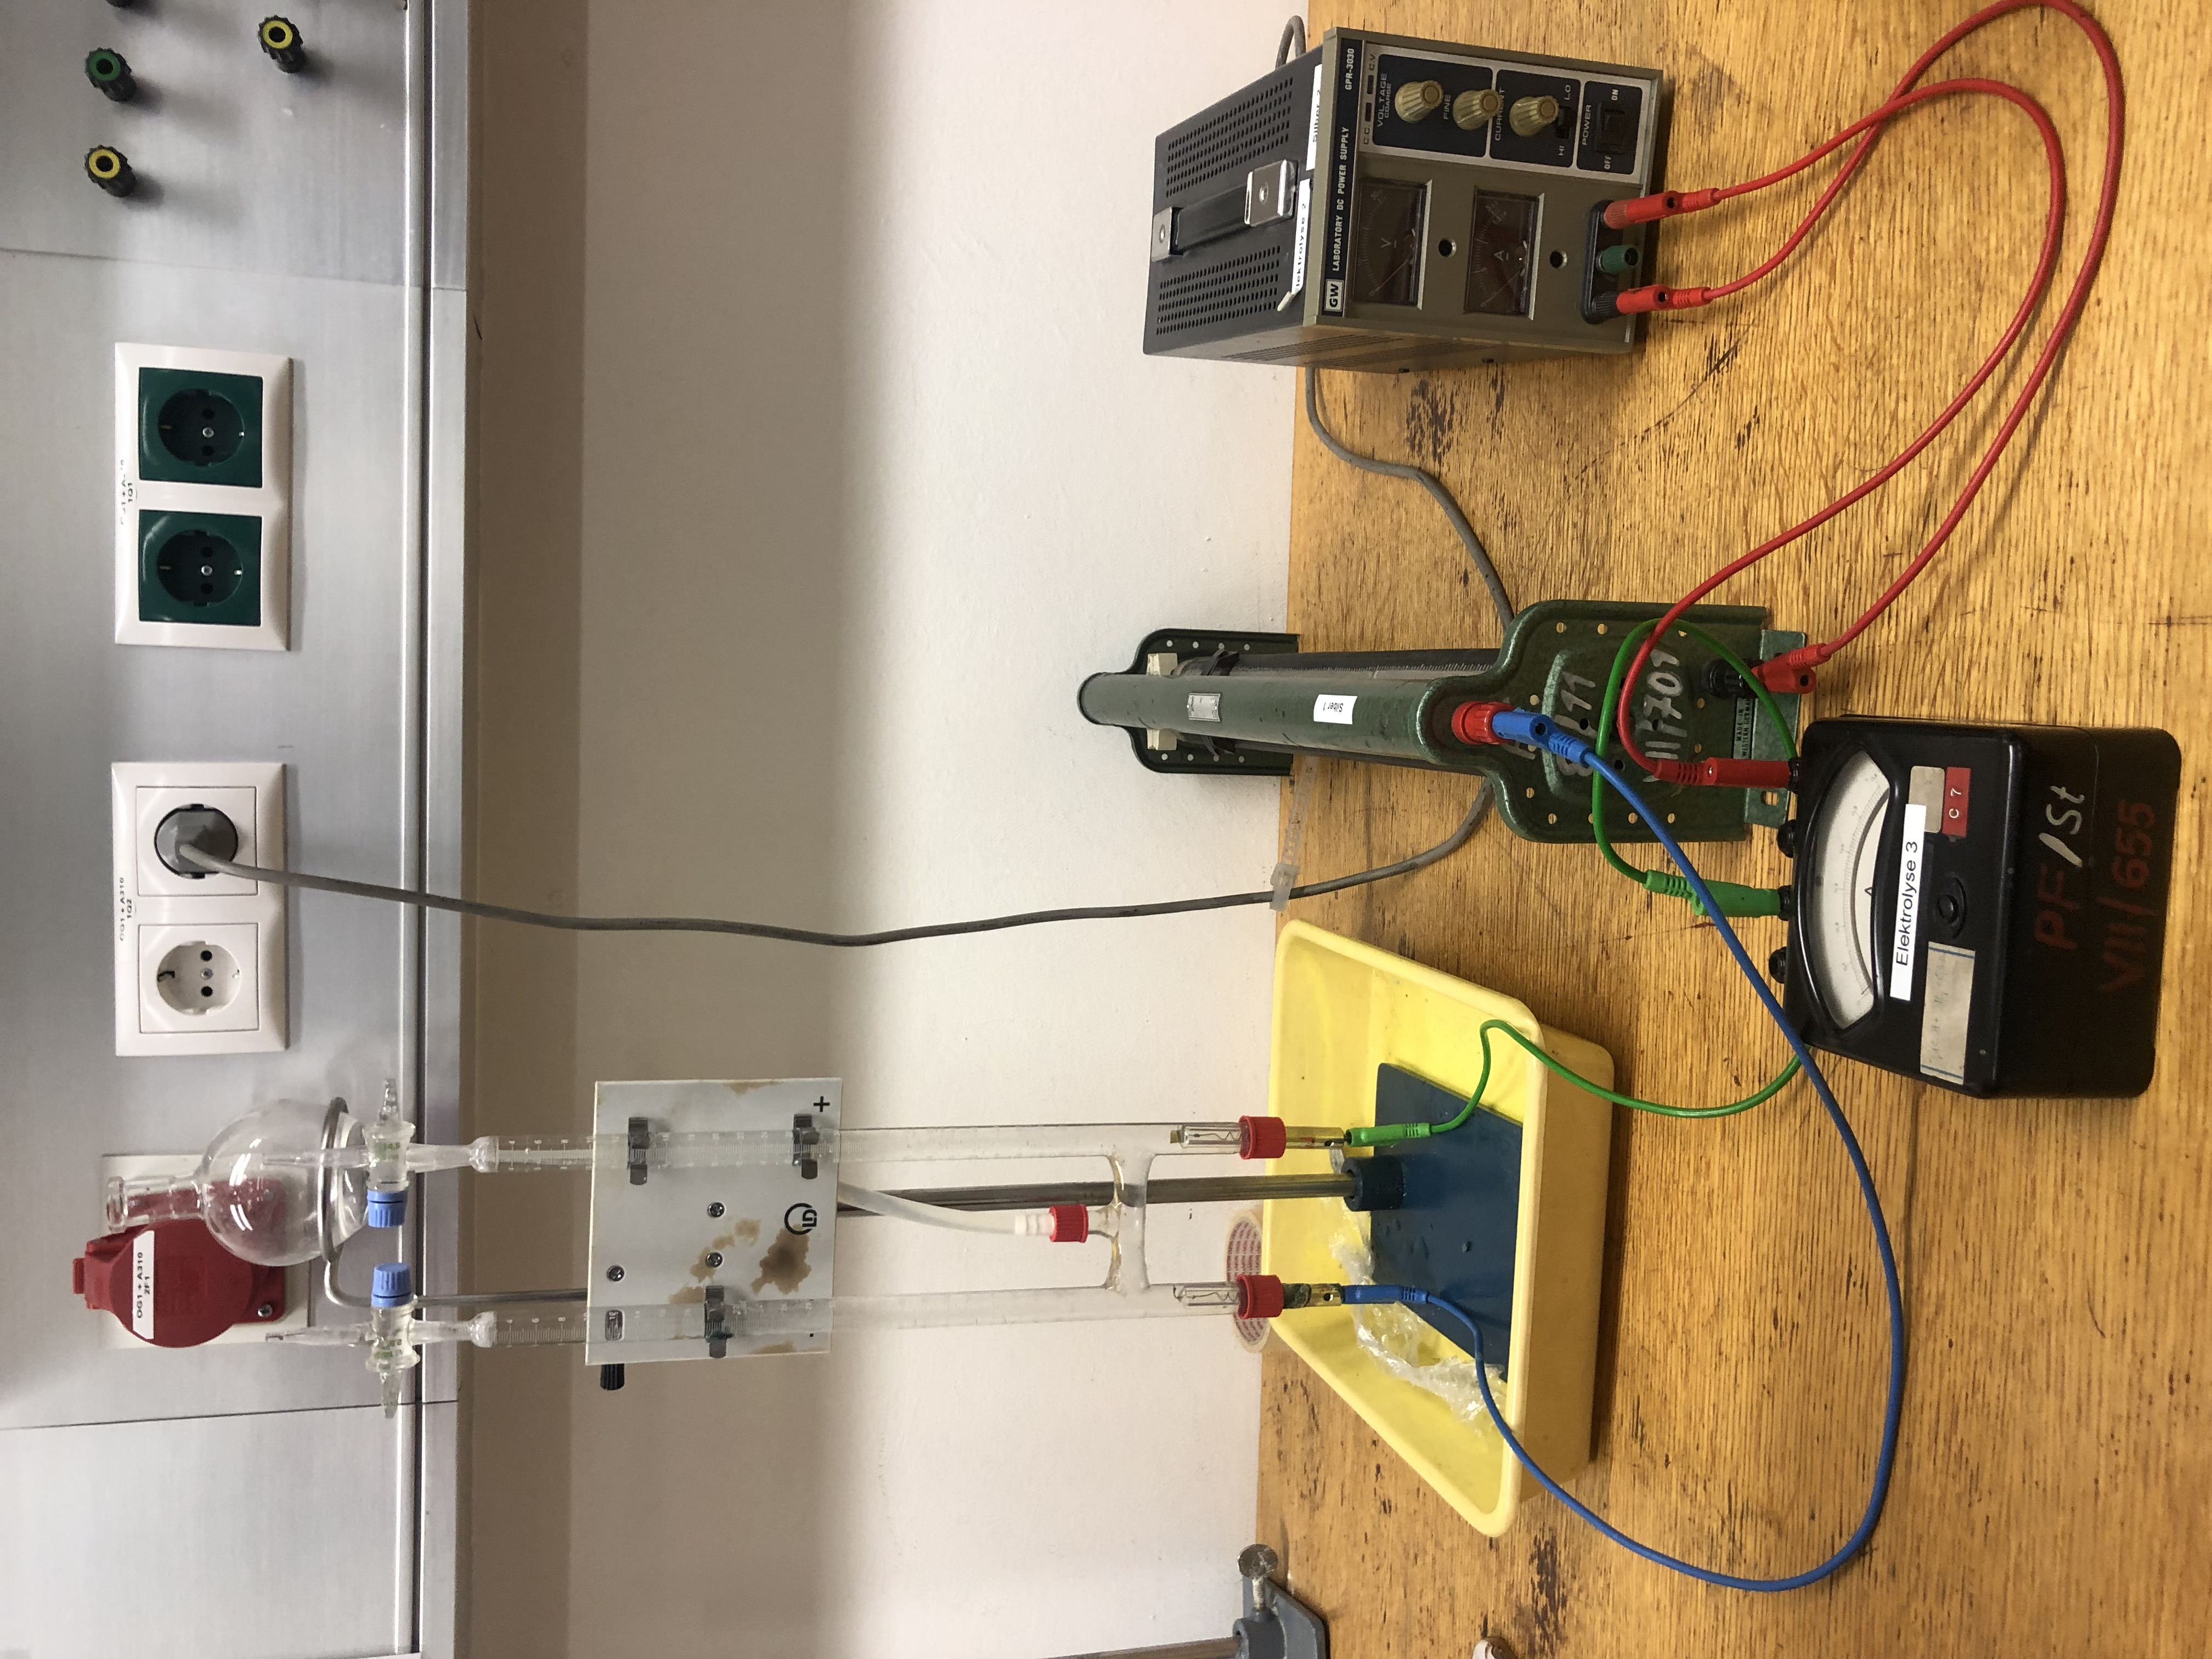
\includegraphics[angle=-90,width=0.5\textwidth]{aufbau_el}
	\end{center}
	\caption{Versuchsaufbau für die Elektrolyse}
	\label{fig:aufbau_el}
\end{figure}\cite{vorlagesilber}

\newpage

\section{Geräteliste}

\noindent Für die Messungen wurden folgende Geräte verwendet:

\captionof{table}{Verwendete Geräte }
\begin{center}
	\begin{tabular}{|c|c|c|c|} \hline
		\textbf{Gerät}             & \textbf{Typ}   & \textbf{Hersteller} \\ \hline

		Gefäß für Silbercoulometer & G17            &                     \\ \hline
		AgNO$_3$                   &                &                     \\ \hline
		Elektroden                 & Silber         &                     \\ \hline
		``Power Supply``           & GPR-1830       & GW                  \\ \hline
		Widerstand                 & 5700 $\Omega$  & R                   \\ \hline
		Amperemeter                & VII/1041/3     &                     \\ \hline
		Kabel                      & Bananenstecker &                     \\ \hline
		Waage                      & P163           & Mettler             \\ \hline
		Stoppuhr                   & Smartphone     &                     \\ \hline
		Schleifpapier              &                &                     \\ \hline
		Gefäß für Elektrolyse      &                &                     \\ \hline
		H$_2$SO$_4$                &                &                     \\ \hline
		Widerstand                 & 75 $\Omega$    & R                   \\ \hline
		Senkspindel                &                &                     \\ \hline
	\end{tabular}
\end{center}


\section{Versuchsdurchführung \& Messergebnisse}\label{sec:Versuchsdurchführung}

Zunächst wird die Raumtemperatur und der aktuelle Luftdruck gemessen, die für den gesamten Versuch benötigt werden. Dadurch ergeben sich folgende Werte:

\begin{align*}
	T = \SI{22(1)}{\degree} \\
	p = \SI{95800(800)}{Pa}
\end{align*}

Dabei ist anzumerken, dass der Luftdruck im Laufe des Versuchs um \SI{200}{Pa} gesunken ist. Dies ist aber aufgrund der hohen Unsicherheit vernachlässigbar.

\subsection{Silbercoulometer}

Zunächst werden die Elektroden mit dem Schleifpapier abgeschmirgelt, um diese von den Resten aus den vorherigen Versuchen zu befreien. Zusätzlich ist darauf zu achten, dass die Aufhängung der Elektroden lang genug ist, um in die Flüssigkeit zu hängen.

\vspace{2mm}

Nun werden die Elektroden abgewogen und die entsprechenden Werte in \autoref{tab:massen} notiert. Bei der Waage der Marke Mettler ist darauf zu achten, dass diese richtig auf ``Tara`` gestellt ist, wie in \autoref{fig:waage} sichtbar, um einen, so zu Stande kommenden systematischen Fehler zu vermeiden. Die Unsicherheit der Masse entsteht durch die Auflösung der Waage und beträgt daher \SI{0.001}{\g}.

\begin{figure}[H]
	\begin{center}
		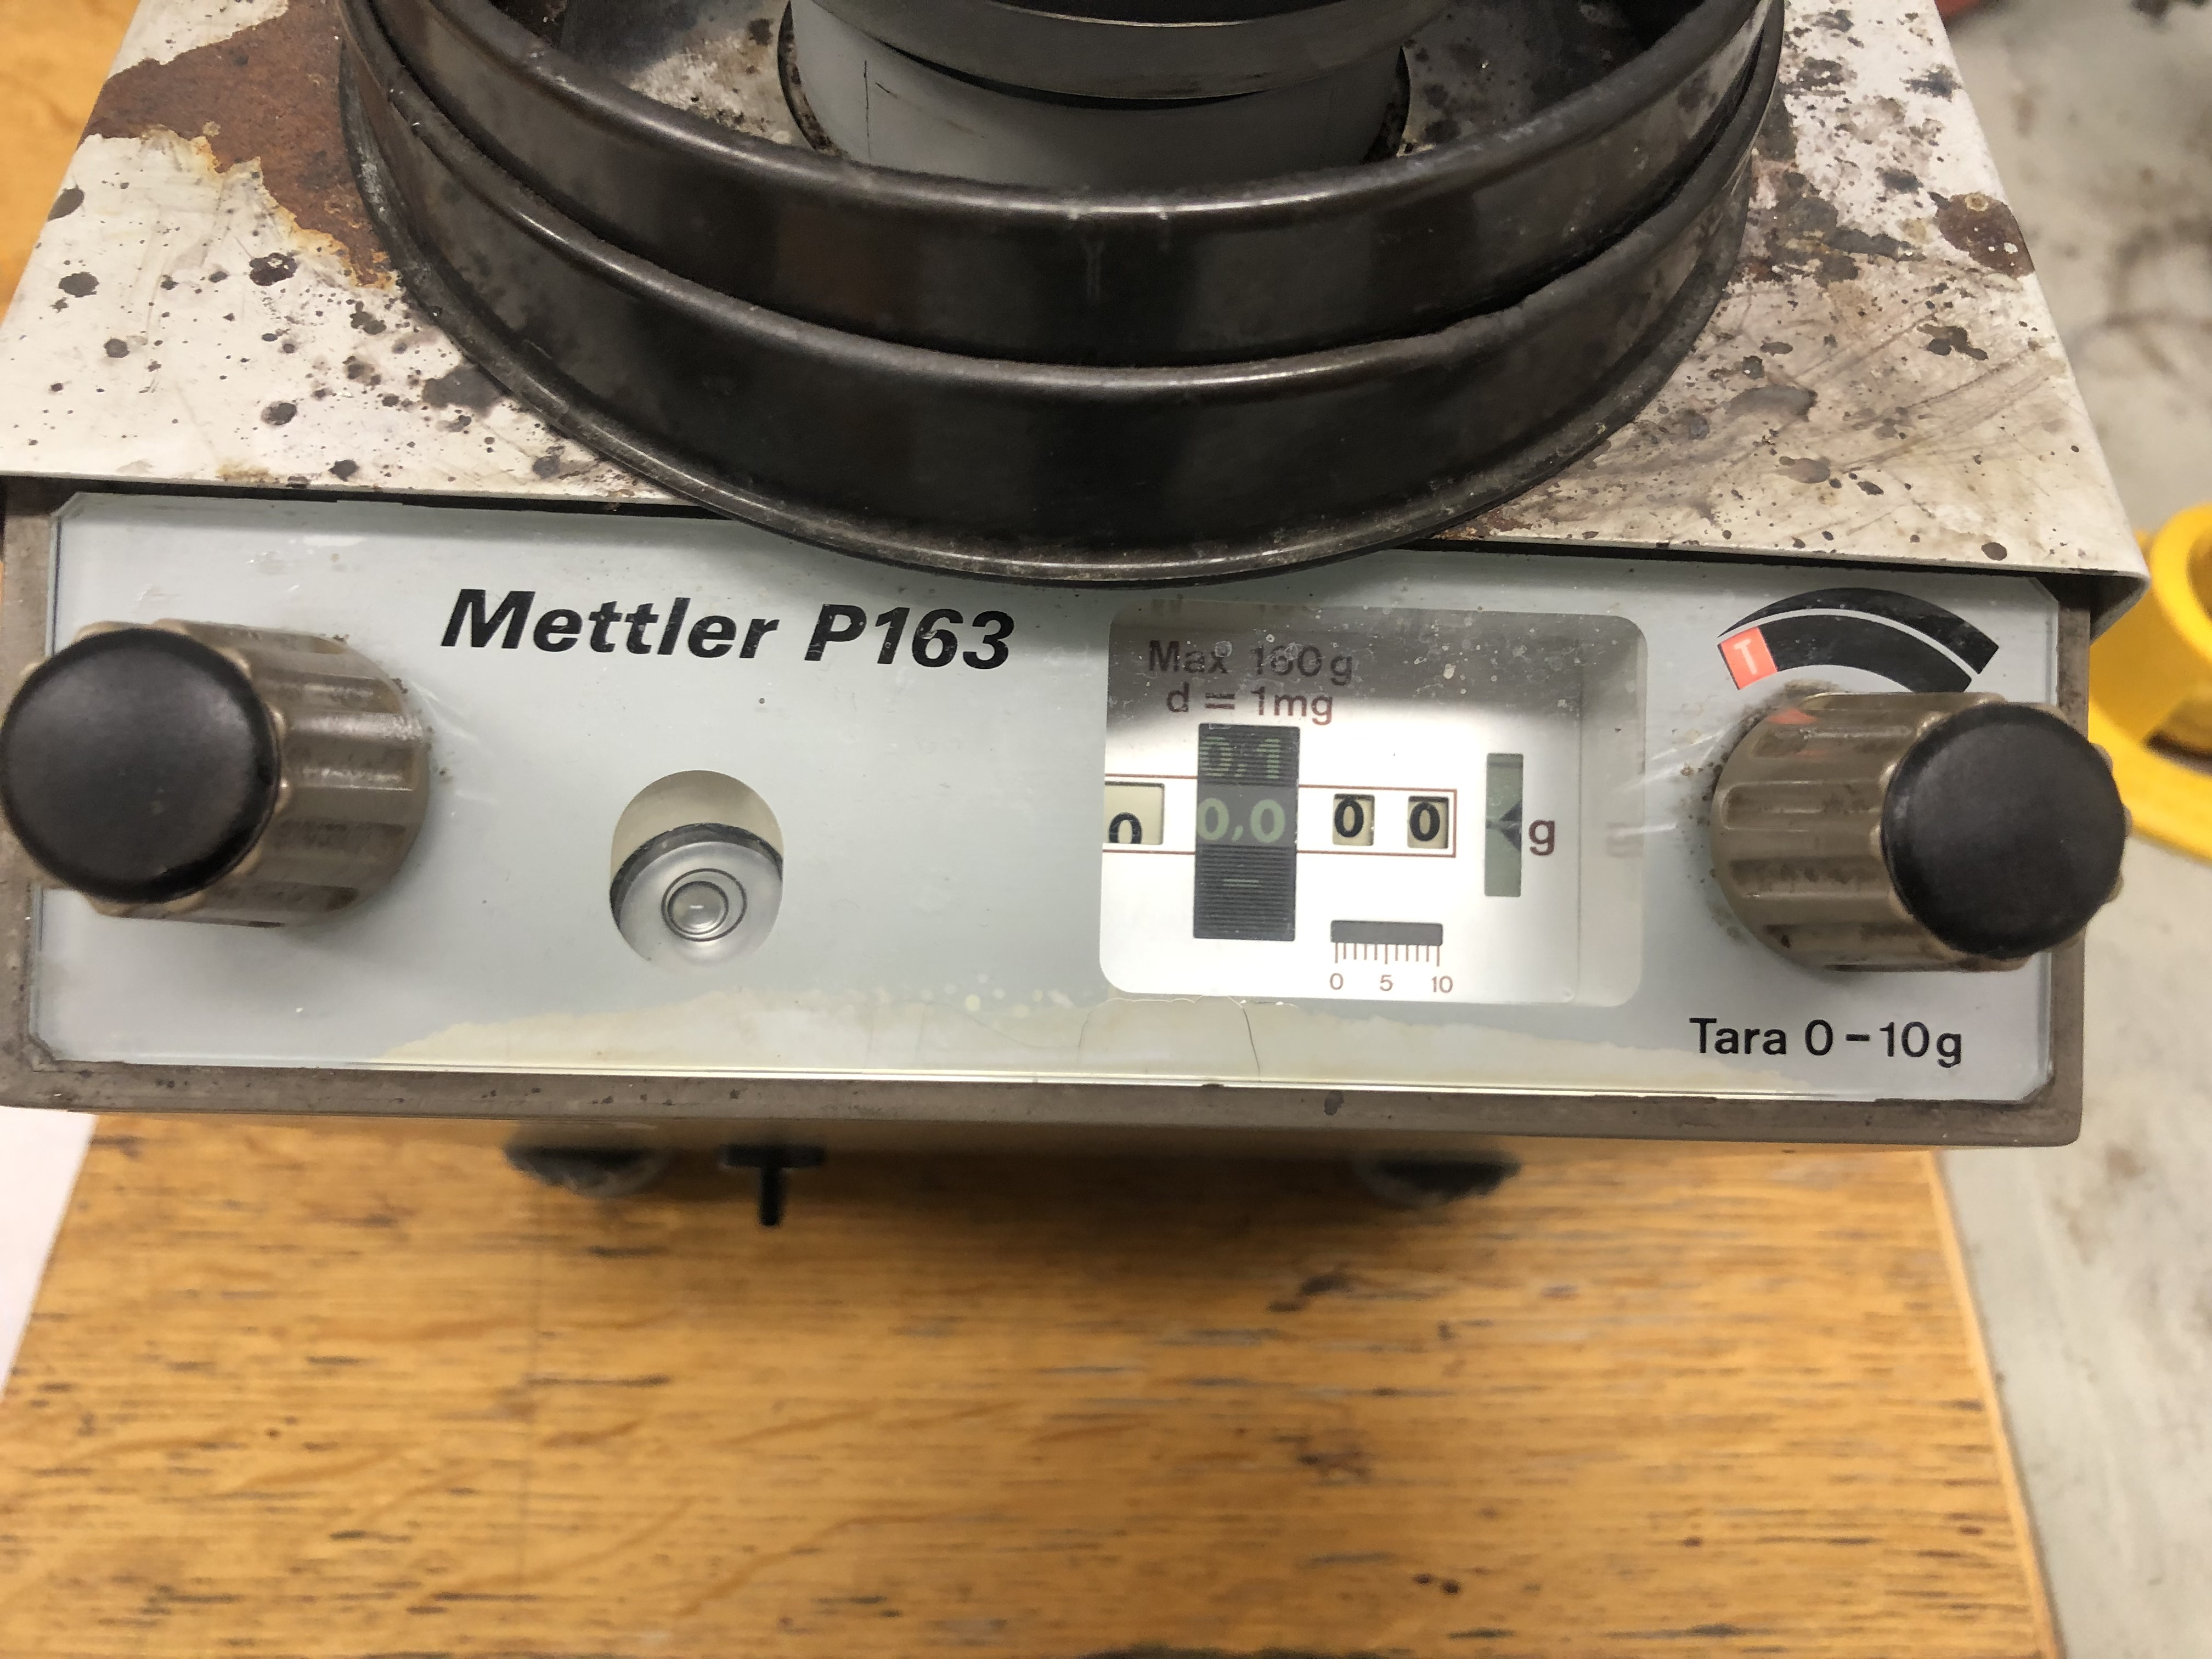
\includegraphics[width=0.5\textwidth]{waage}
	\end{center}
	\caption{``Tara``- Stellung der Waage}
	\label{fig:waage}
\end{figure}

Nun werden die Elektroden, wie in \autoref{fig:aufbau_ag} sichtbar in die AgNO$_3$ Lösung gehängt und der ``Power Supply`` eingeschalten. Zeitgleich dazu wird auch die Smartphone-Stoppuhr gestartet, um die genaue Zeit festzustellen. Mithilfe des in Serie geschalteten Amperemeters kann überprüft werden, dass der fließende Strom stets einen konstanten Wert von \SI{100(4)}{mA} beträgt.

Über die Dauer des Versuchs sinkt, durch die Erwärmung der Flüssigkeit, der Widerstand der AgNO$_3$ Lösung, wie bereits in den Grundlagen erwähnt, weshalb auch die Spannung angepasst werden muss, um einen konstanten Strom zu gewähren.

\vspace{2mm}

Nach einer Versuchszeit von \SI{3600(1)}{\s} wird der Strom abgeschaltet und die Elektroden vorsichtig aus der Lösung entfernt. Dabei ist vor allem darauf zu achten, möglichst keine Ablagerungen der Kathode zu verlieren. Dies ist leider nicht gelungen und der Dendrit, welcher entstanden und in \autoref{fig:dendrit} ersichtlich ist, konnte leider nicht mit ``geborgen`` werden. Der ``Anodenschlamm`` wird nun vorsichtig abgewischt und die beiden Elektroden trockengeföhnt, um sicherzustellen, dass kein Wasser mit gewogen wird. Die Silberablagerungen an der Kathode sind in \autoref{fig:elektroden} ersichtlich.

\begin{minipage}{\textwidth}
	\begin{minipage}[t]{0.5\textwidth}
		\centering
		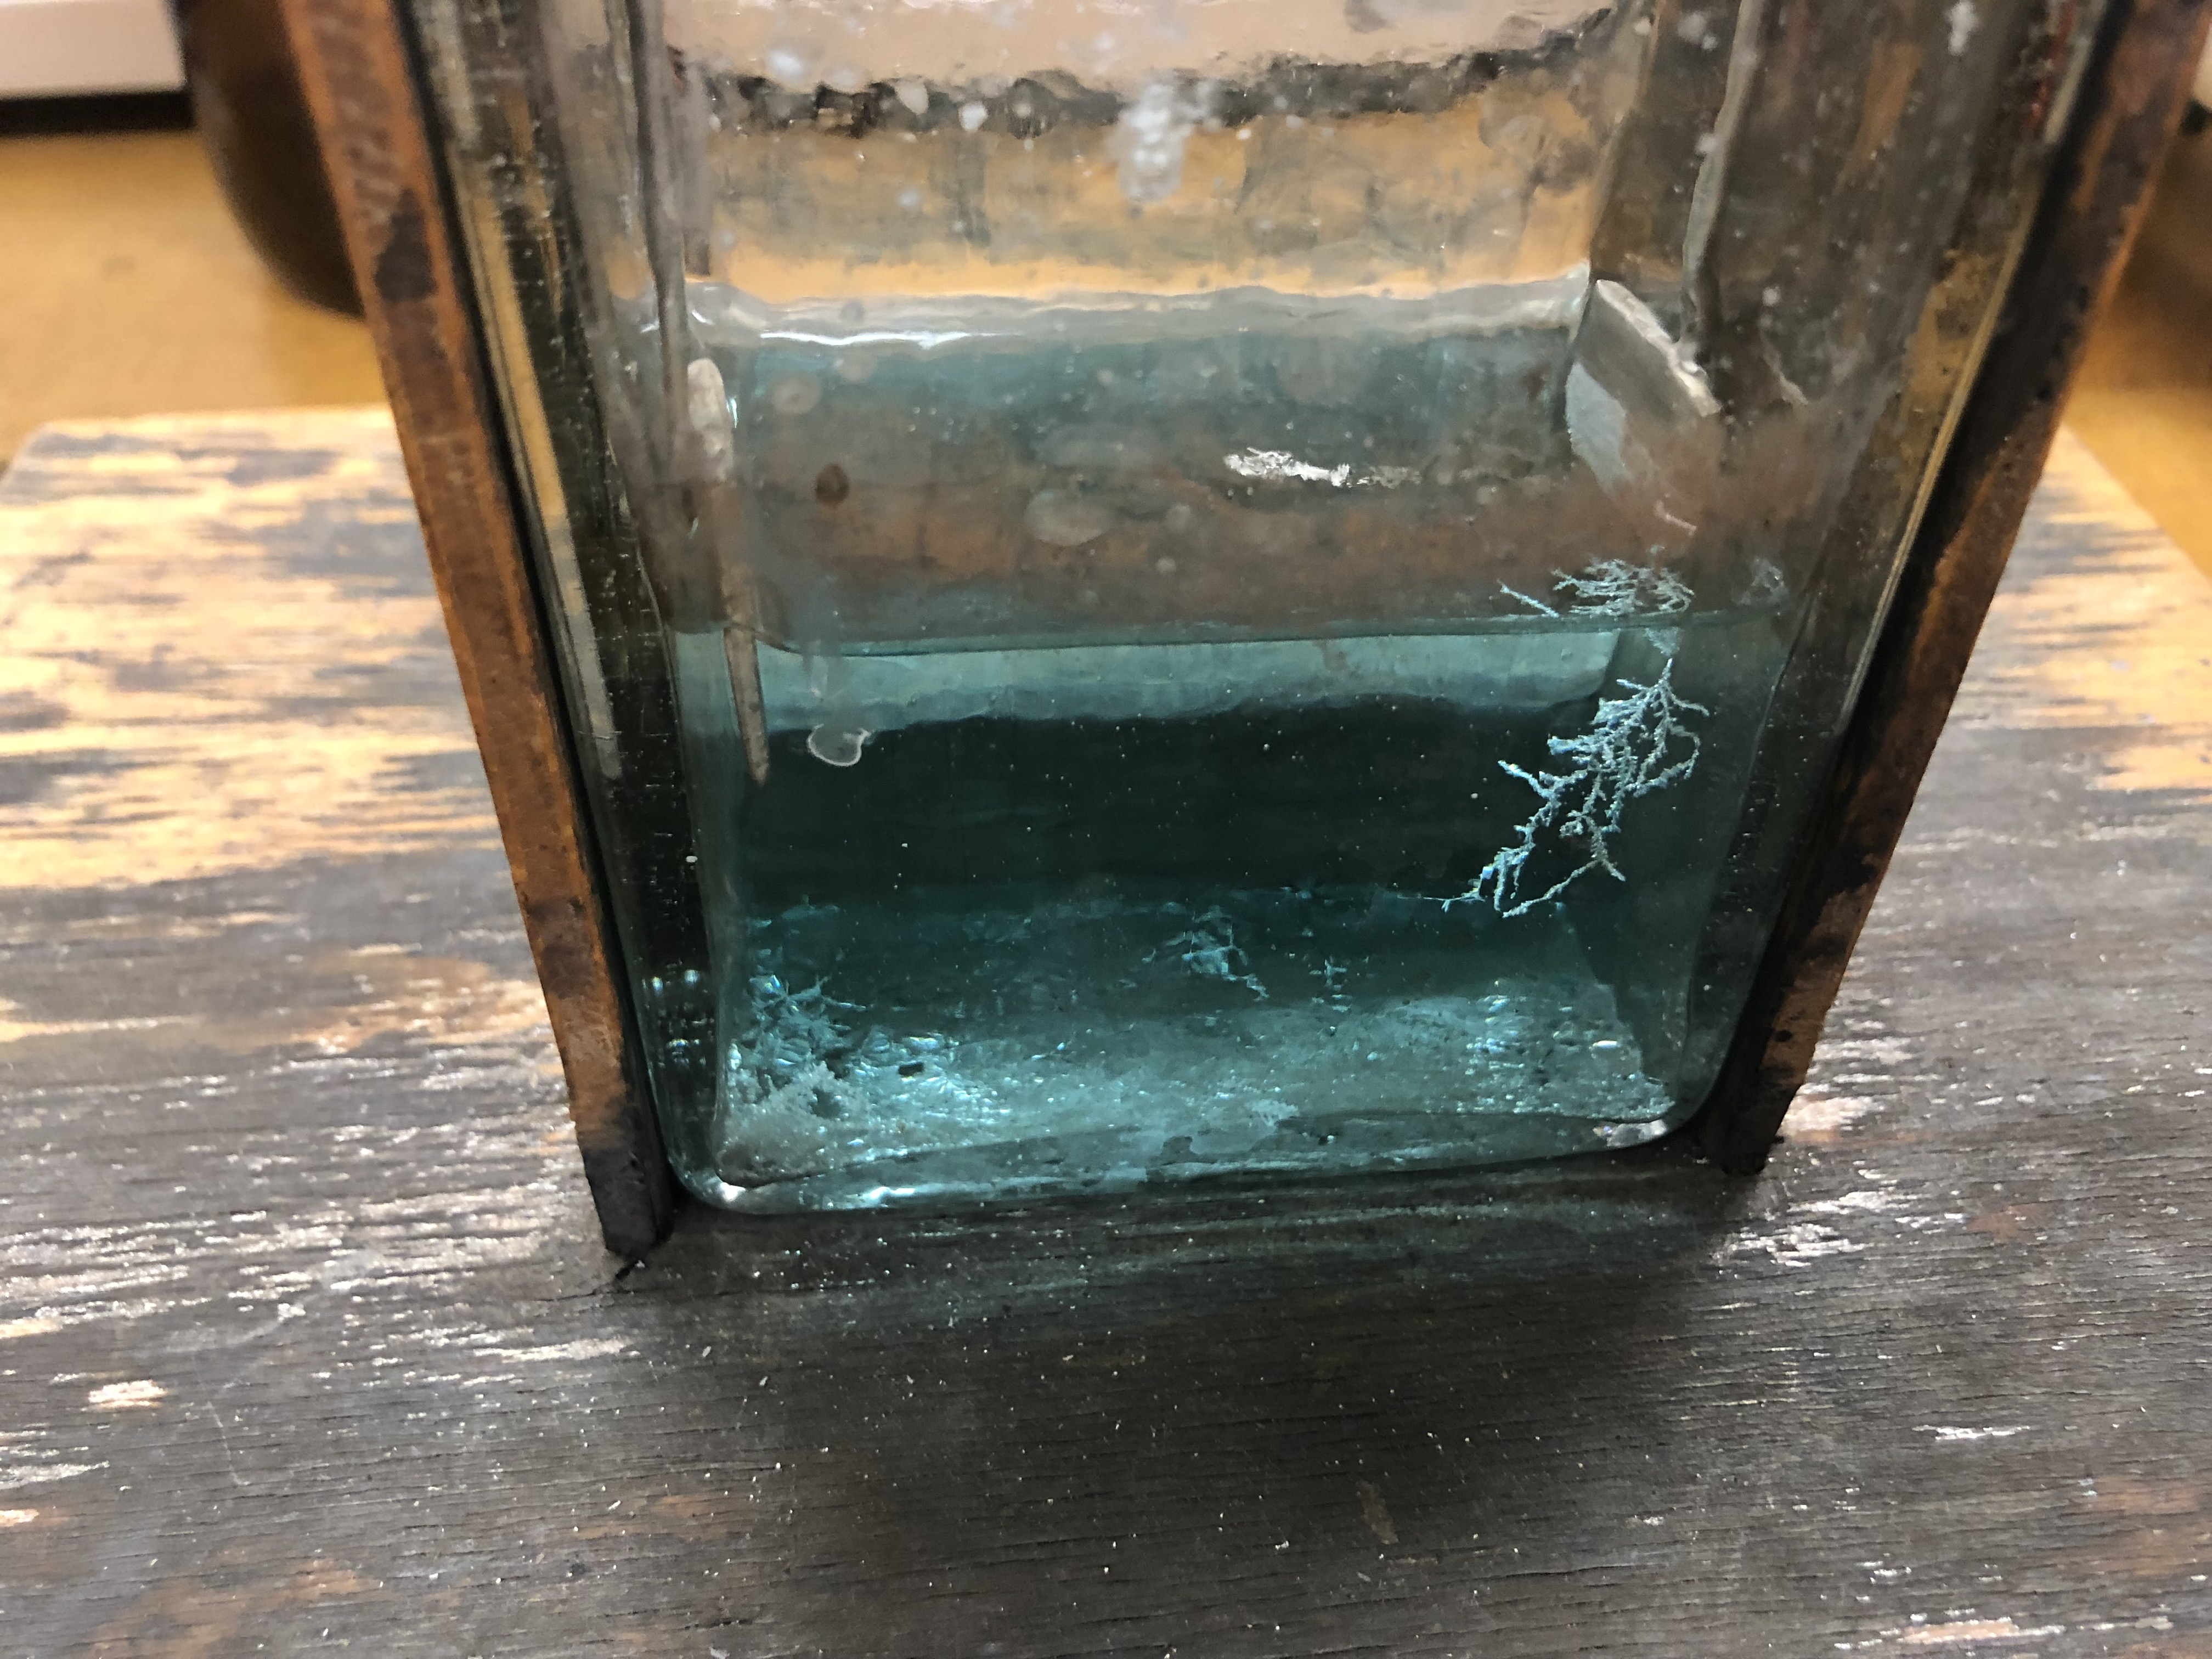
\includegraphics[width=\textwidth]{dendrit}
		\captionbelowof{figure}{gebildeter Dendrit an der Kathode}
		\label{fig:dendrit}
	\end{minipage}
	\vspace{2mm}
	\begin{minipage}[t]{0.50\textwidth}
		\centering
		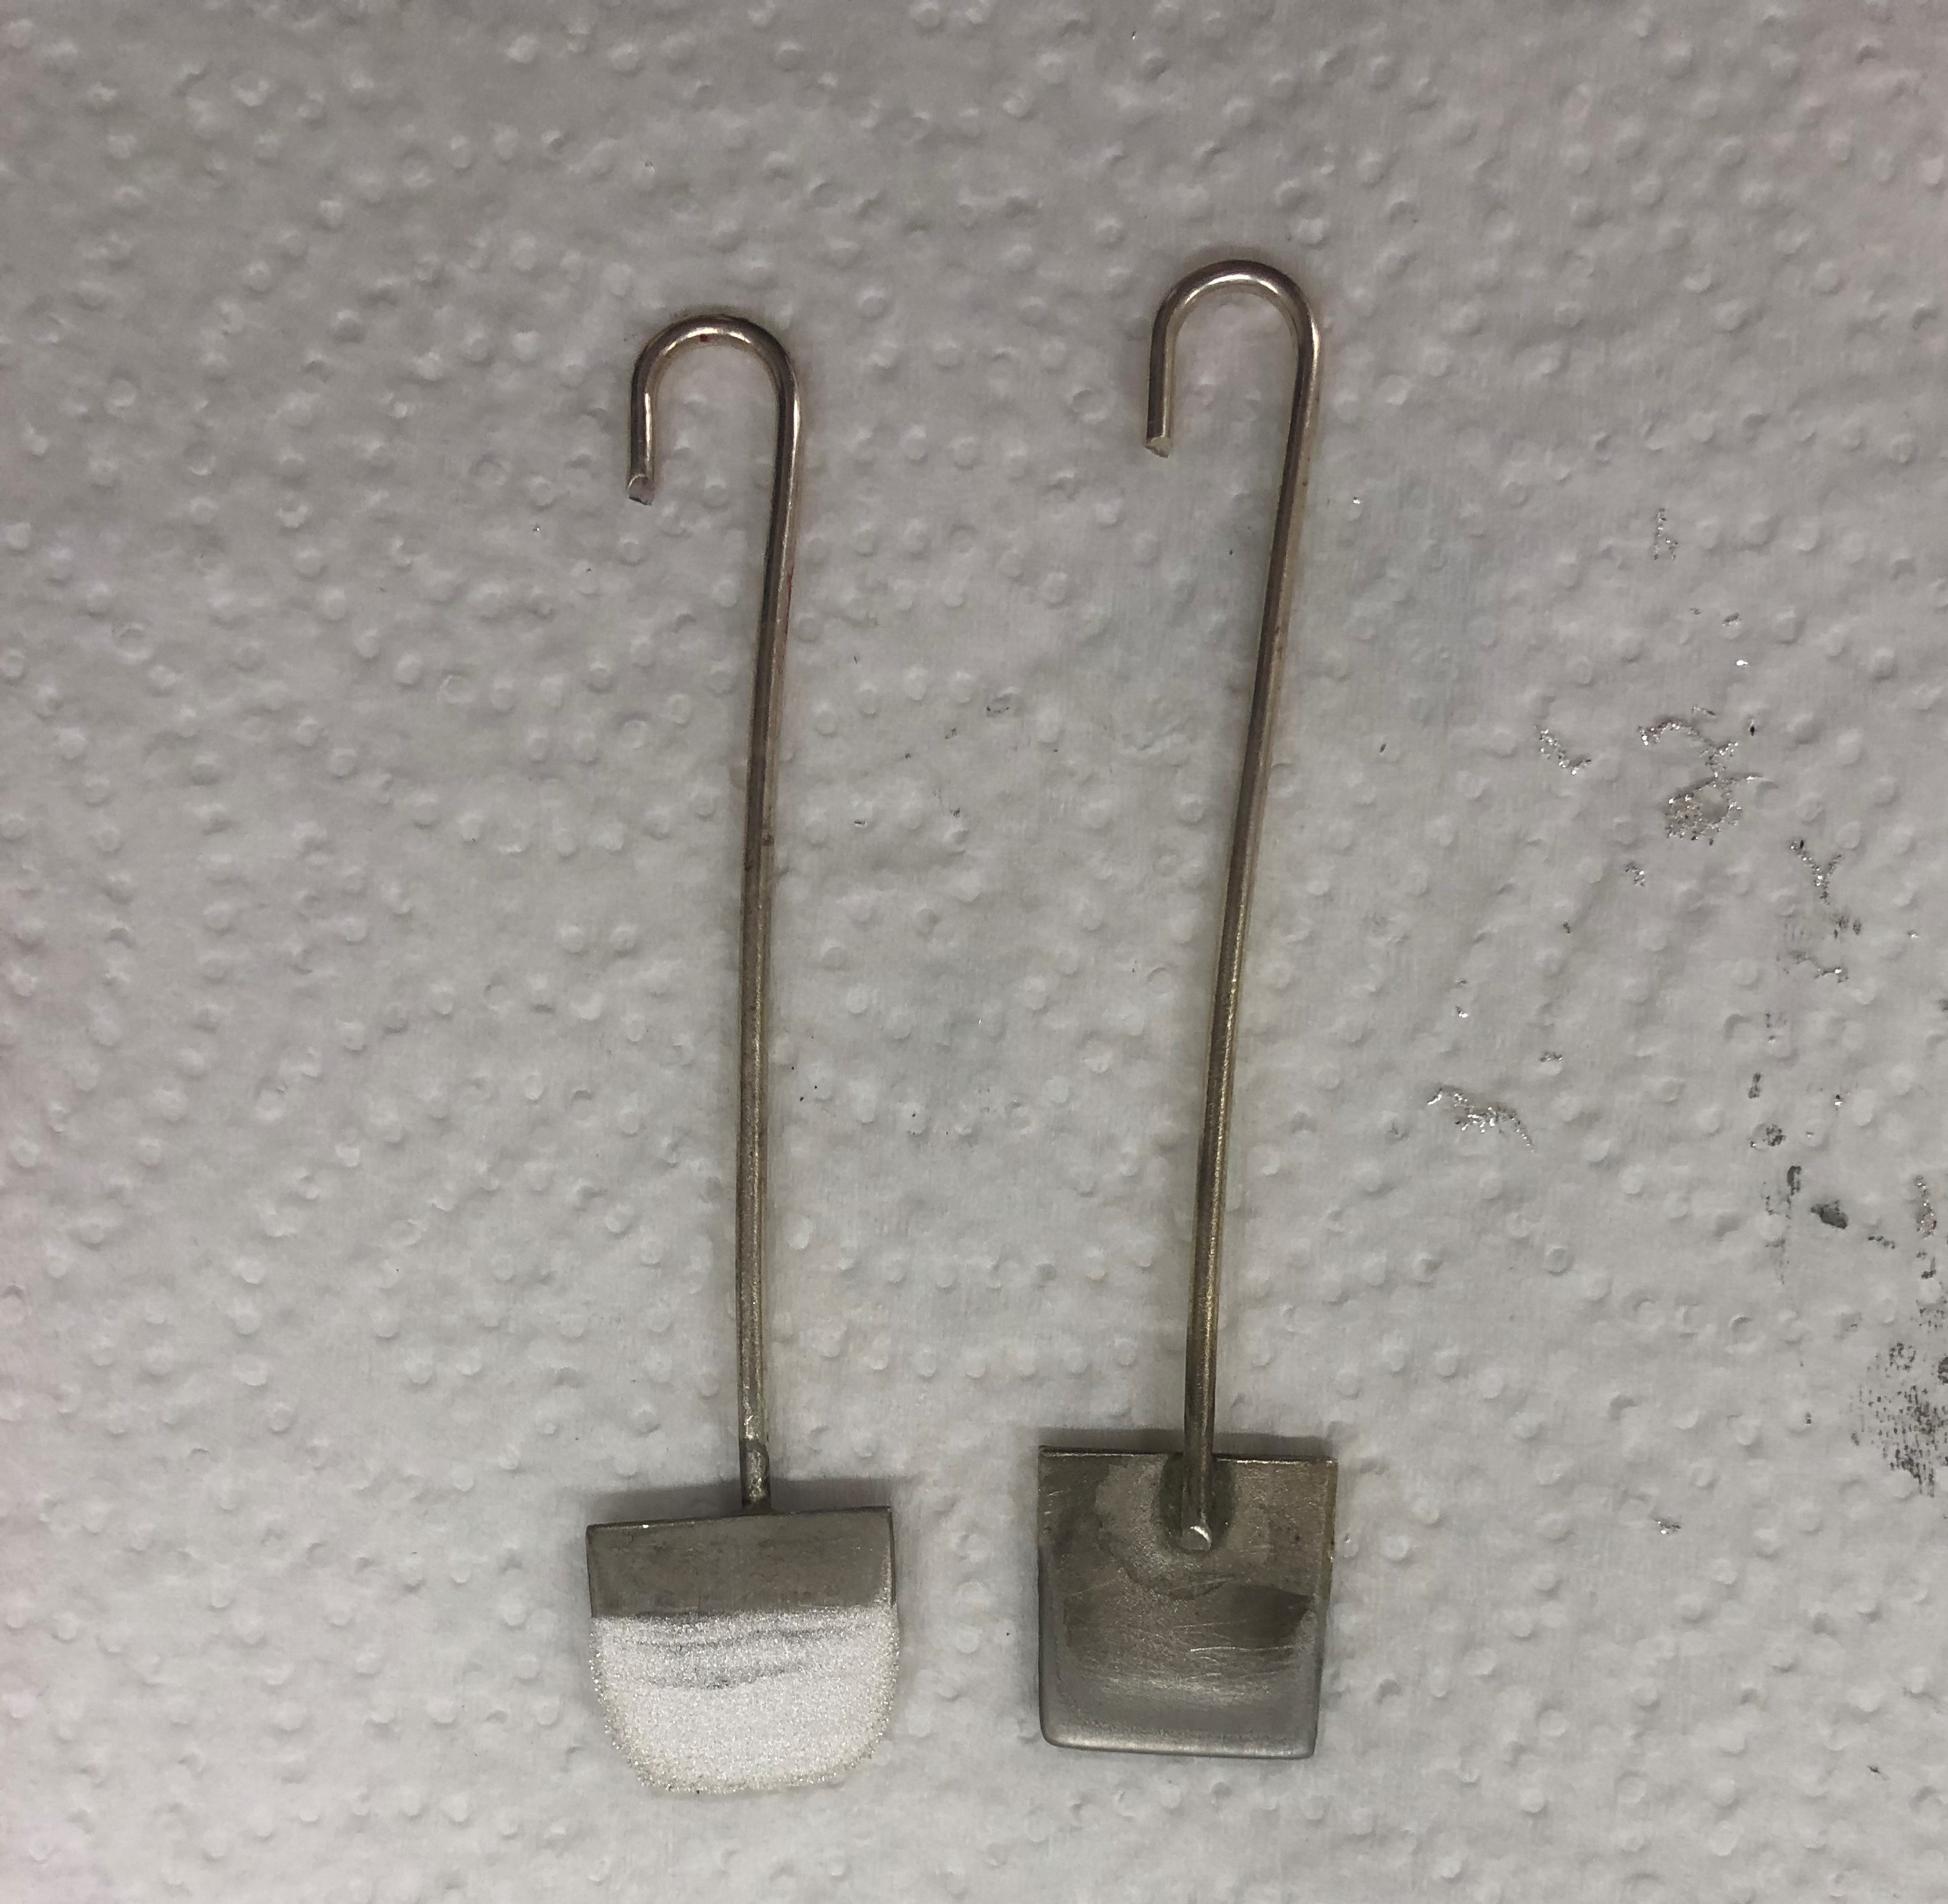
\includegraphics[width=\textwidth]{elektroden_neu}
		\captionof{figure}{Silberablagerungen sichtbar auf der Kathode (links)}
		\label{fig:elektroden}
	\end{minipage}
	\vspace{1em}
\end{minipage}

Die erhaltenen Massen vor und nach dem chemischen Prozess sind in folgender Tabelle angeführt:

\captionof{table}{abgelesene Massen der Elektroden\\
	A $\dots$ Anode \\
	K $\dots$ Kathode \\
	$m_v \dots$ abgelesene Masse vor dem Prozess \\
	$m_n \dots$ abgelesene Masse nach dem Prozess }
\begin{center}
	\begin{tabular}{|c|S[table-format=2.3(1)]|S[table-format=2.3(1)]|} \hline
		  & {$m_v$ / g} & {$m_n$ / g} \\ \hline
		A & 10,832	(1)   & 10,474	(1)   \\ \hline
		K & 8,438(1)    & 8,691(1)    \\ \hline
	\end{tabular}
	\label{tab:massen}
\end{center}



\subsection{Elektrolyse}

Beim zweiten Teil des Versuchs muss die Dichte der H$_2$SO$_4$ Lösung bestimmt werden. Dazu wird diese in ein Gefäß gefüllt und eine passende Senkspindel in dieses gelegt, sodass die Senkspindel, wie in \autoref{fig:ente} ersichtlich, schwimmt und die Spindel nicht zu Boden sinkt. Die verschiedenen Senkspindeln in \autoref{fig:senkspindeln} sind mit einer unterschiedlichen Menge an Blei gefüllt, sodass die Dichte der Lösung anhand der entsprechenden Skala auf der Senkspindel an der Position des Lösungsstands abgelesen werden kann.

Dadurch ergibt sich folgende Dichte $\rho$:

\begin{align*}
	\rho = \SI{1110(4)}{\g\per\L}
\end{align*}


\begin{minipage}{\textwidth}
	\begin{minipage}[t]{0.49\textwidth}
		\centering
		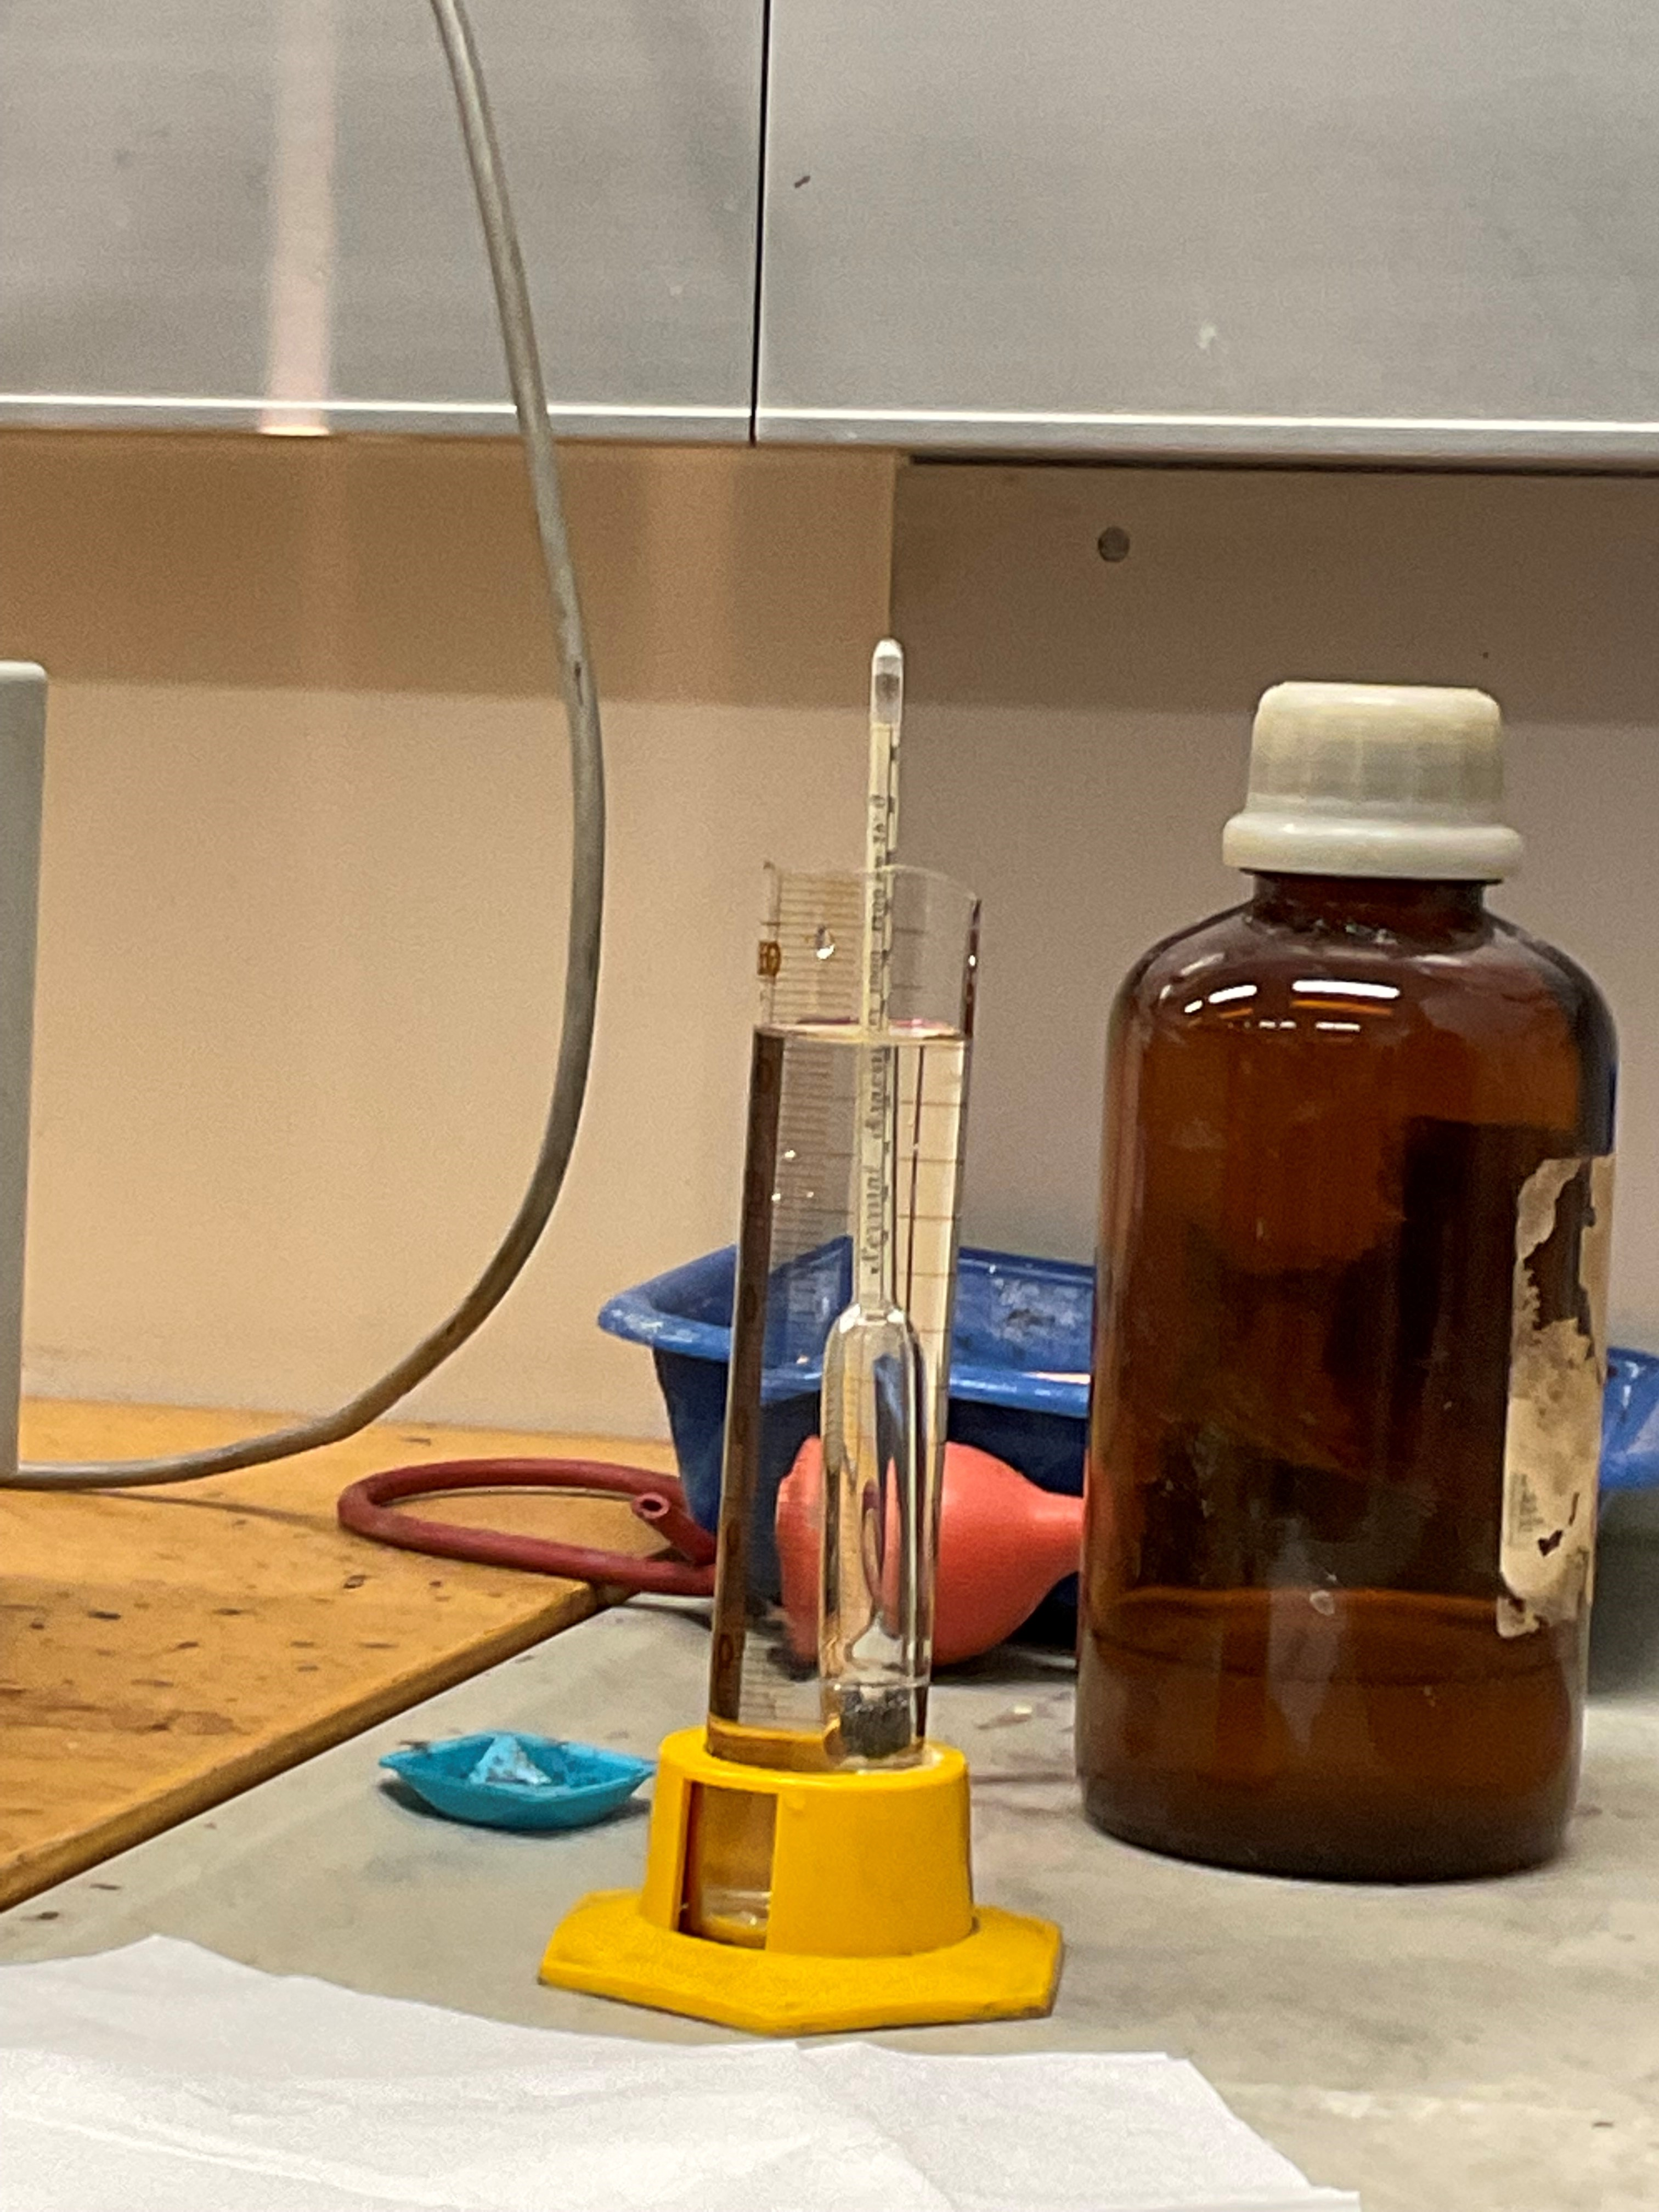
\includegraphics[width=\textwidth]{ente}
		\captionbelowof{figure}{passende Senkspindel, die in der Flüssigkeit schwimmt}
		\label{fig:ente}
	\end{minipage}
	\vspace{2mm}
	\begin{minipage}[t]{0.49\textwidth}
		\centering
		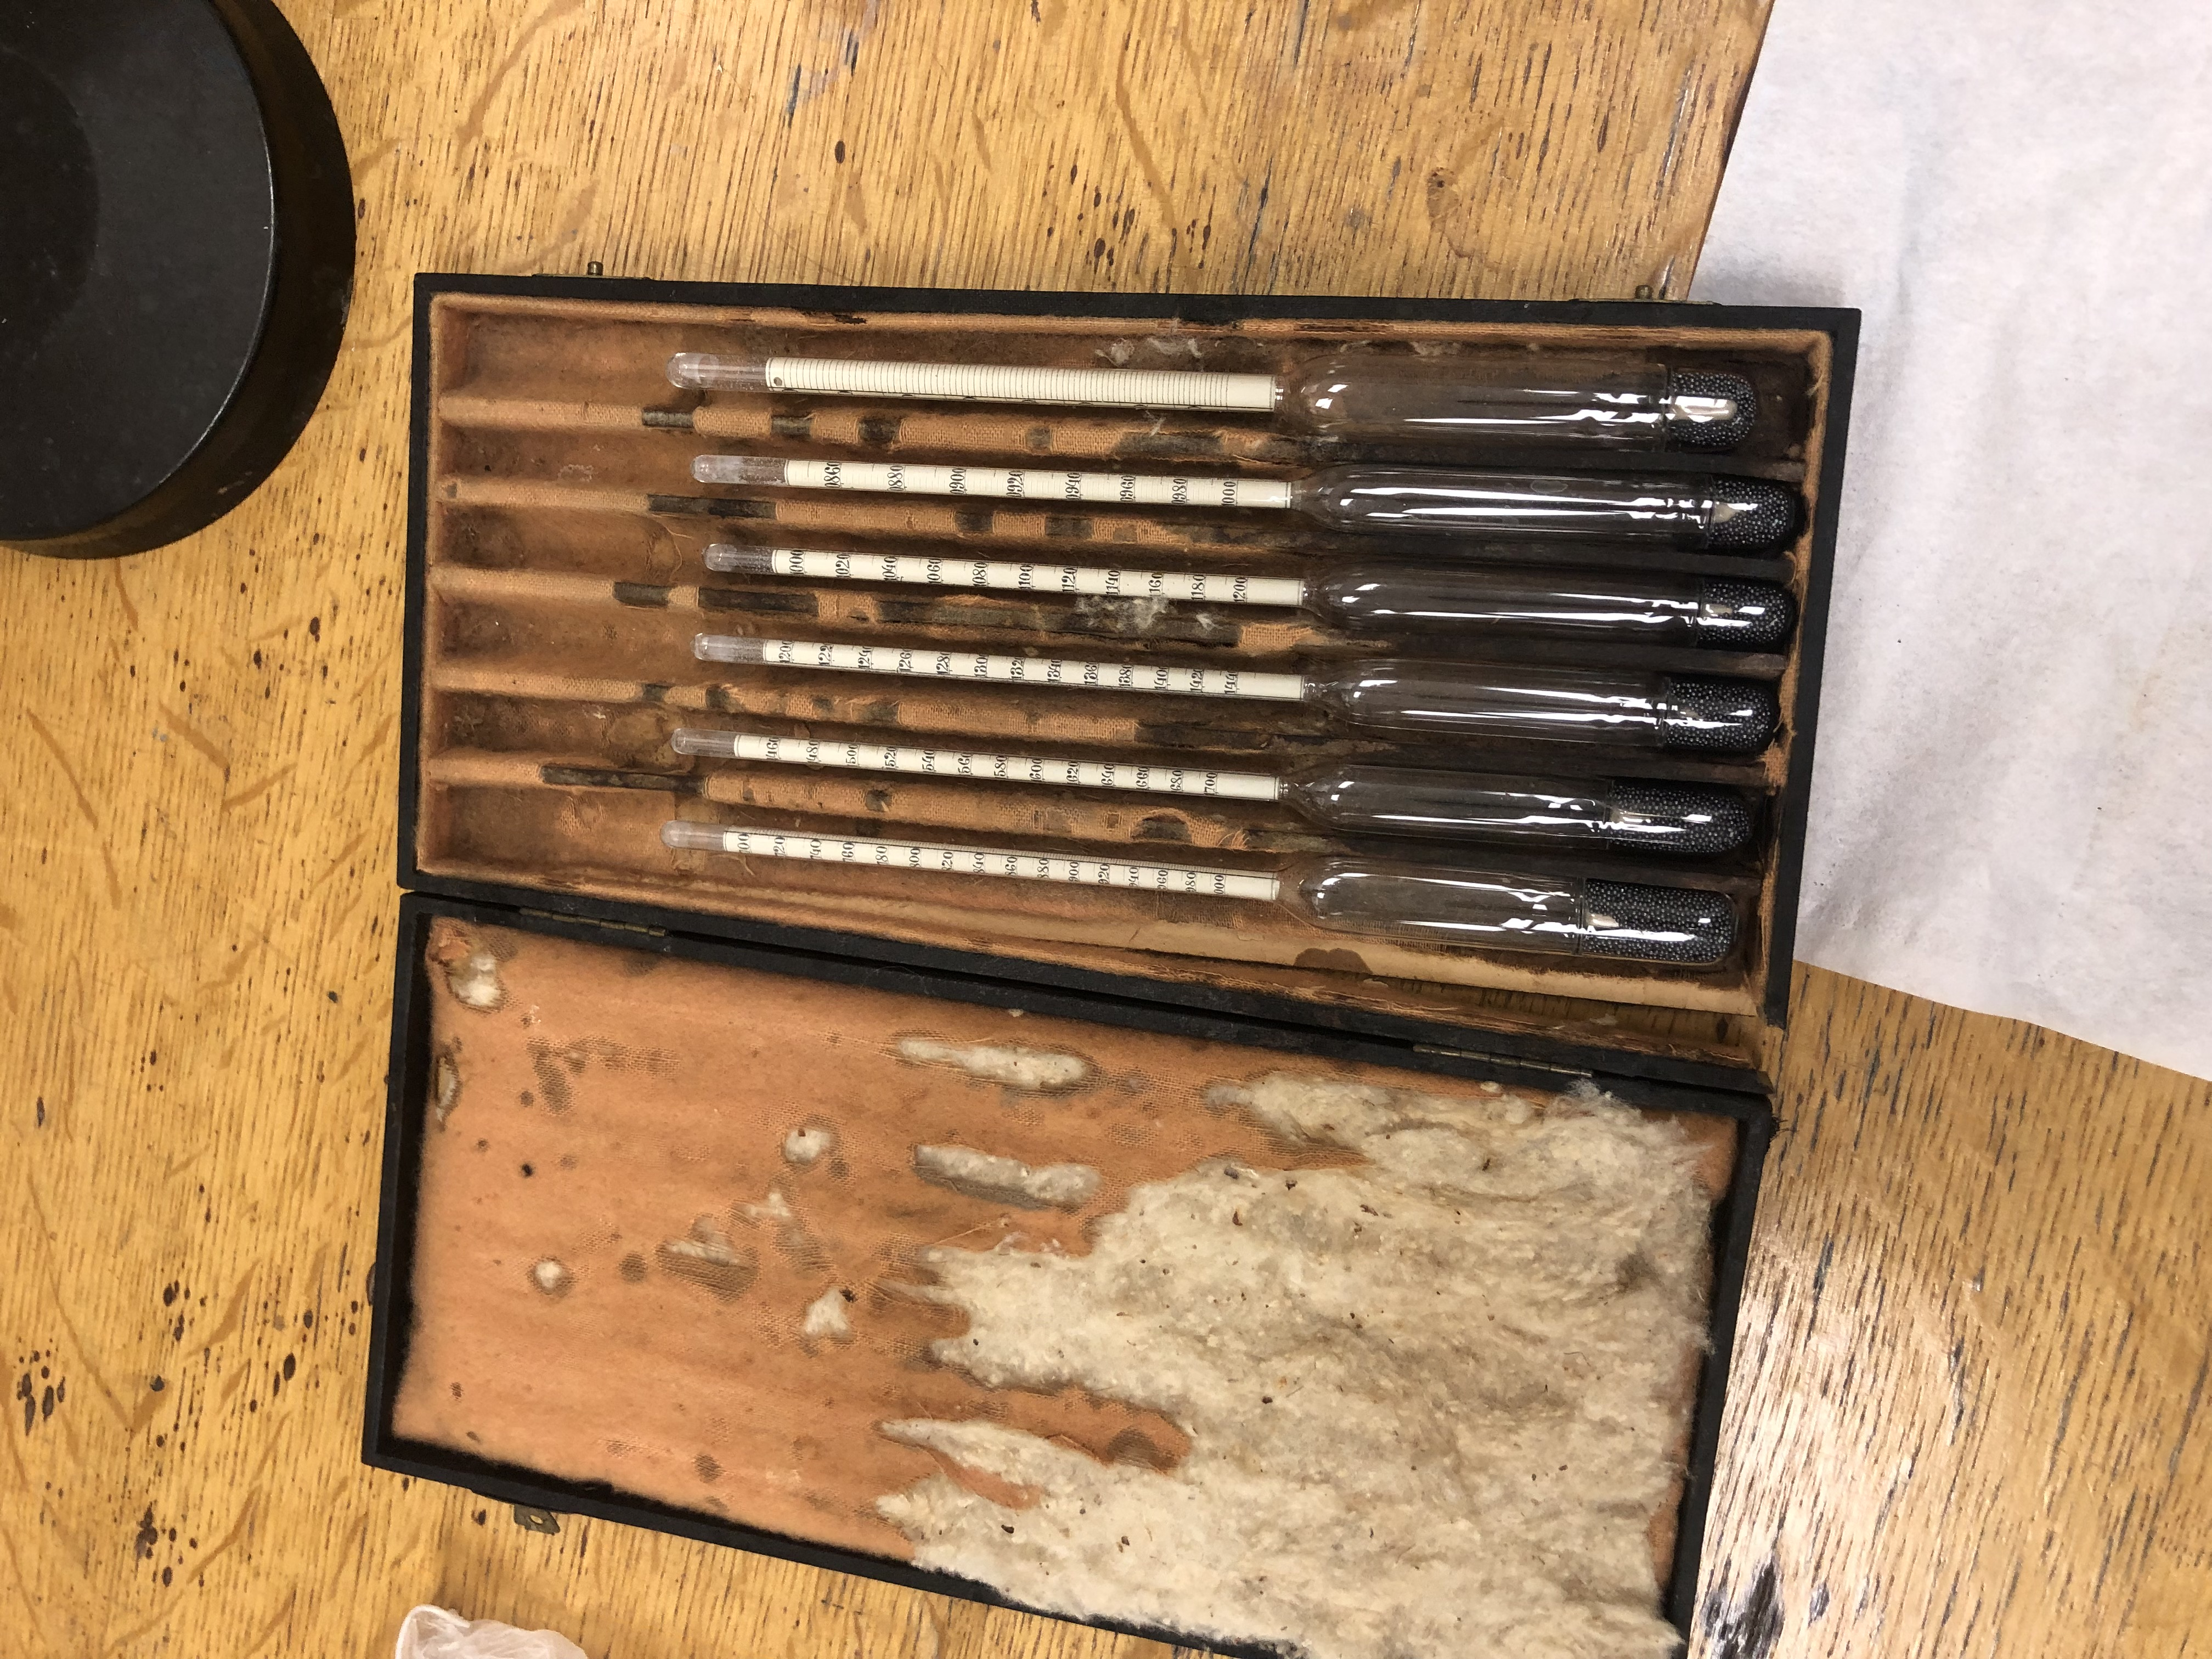
\includegraphics[angle=90,width=\textwidth]{senkspindeln}
		\captionof{figure}{verschiedene Senkspindeln}
		\label{fig:senkspindeln}
	\end{minipage}
	\vspace{1em}
\end{minipage}

Nun wird der Versuch, wie in \autoref{fig:aufbau_el} ersichtlich, aufgebaut.

Zunächst wird die Stromversorgung kurz eingeschalten, um dafür zu sorgen, dass der Flüssigkeitsstand in beiden Röhrchen auf einen Wert sinkt, der mithilfe der Skala abgelesen werden kann. Dies wird nun durchgeführt und die so erhaltenen Werte in folgender \autoref{tab:el_1} notiert. Nun wird die Elektrolyse für eine Zeit von $t=\SI{600(1)}{\s}$ bei einem konstanten Strom von \SI{0.300(4)}{A}, der mithilfe des in Serie geschalteten Amperemeters überprüft wird, durchgeführt. Die Zeit wird, wie zuvor, mithilfe der Smartphone Stoppuhr überprüft.

\vspace{2mm}

Nun werden erneut die Werte des Flüssigkeitsstands abgelesen und in folgender Tabelle notiert. Auch wird die Höhendifferenz zwischen dem Ausgleichsbehälter und der Flüssigkeitshöhe zwischen den beiden Röhren mit einem Lineal ermittelt. Da dies bei der entsprechenden Versuchsanordnung nur äußerst ungenau möglich ist, wird die Ungenauigkeit auf \SI{1}{\cm} geschätzt.

\newpage

\captionof{table}{abgelesene Daten der Elektrolyse bei einer Zeit von \SI{600(1)}{\s} und einem Strom von \SI{0.300(4)}{A} \\
	$V_{0} \dots$ Volumen vor der Elektrolyse\\
	$V_{e} \dots$ Volumen nach der Elektrolyse\\
	h $\dots$ Höhendifferenz \\
	$L \dots$ Linkes Röhrchen \\
	$R \dots$ Rechtes Röhrchen }
\begin{center}
	\begin{tabular}{|c|S[table-format=1.1(1)]|S[table-format=2.1(1)]|S[table-format=2(1)]|} \hline
		  & {$V_{0}$ / mL} & {$V_{e}$ / mL} & {h / cm} \\ \hline
		L & 5,5(4)         & 30,2(4)        & 24(1)    \\ \hline
		R & 2,8(4)         & 14,8(4)        & 16(1)    \\ \hline
	\end{tabular}
	\label{tab:el_1}
\end{center}


Der gesamte Versuch wird nun erneut für eine Zeit von $t=\SI{540(1)}{\s}$ und einen Strom von \SI{0.400(4)}{A} wiederholt, was folgende Werte aus \autoref{tab:el_2} leifert.

\captionof{table}{abgelesene Daten der Elektrolyse bei einer Zeit von \SI{540(1)}{\s} und einem Strom von \SI{0.400(4)}{A} \\
	$V_{0} \dots$ Volumen vor der Elektrolyse\\
	$V_{e} \dots$ Volumen nach der Elektrolyse\\
	h $\dots$ Höhendifferenz \\
	$L \dots$ Linkes Röhrchen \\
	$R \dots$ Rechtes Röhrchen }
\begin{center}
	\begin{tabular}{|c|S[table-format=1.1(1)]|S[table-format=2.1(1)]|S[table-format=2(1)]|} \hline
		  & {$V_{0}$ / mL} & {$V_{e}$ / mL} & {h / cm} \\ \hline
		L & 3,4(4)         & 32,6(4)        & 23(1)    \\ \hline
		R & 3,2(4)         & 18,0(4)        & 14(1)    \\ \hline
	\end{tabular}
	\label{tab:el_2}
\end{center}


\section{Auswertung}

\noindent Um zu sehen wie sich die Unsicherheit der Messungen bis in die Ergebnisse
fortplanzt, ist \autoref{eq:Unsicherheitsfortpflanzung} verwendet worden.
Die Grundlagen dieser Gleichung stammen von den Powerpointfolien von
GUM.\cite{WolfgangKessel2004} Die Verallgemeinerung ist von Wikipedia entnommen
worden \cite{2020Fehler}.
Für die Auswertung ist die Progammiersprache Python im speziellen das
Packet \verb#scipy#, zur Hilfe genommen worden.

\begin{equation}
	\label{eq:Unsicherheitsfortpflanzung}
	V_y = J(x) \cdot V_x \cdot J^{T}(x)
\end{equation}

\noindent Wobei $V_y$ und $V_x$ die Kovarianzmatrizen von den Vektoren $\bm{y}$ und $\bm{x}$ sind.
$\bm{x}$ ist der Vektor der Eingangsvariablen und $\bm{y}$ ist der Vektor der Ausgangsvariablen.
$J$ ist die Jakobimatrix der vektorwertigen Funktion $\bm{y} = \vec{F}(\bm{x})$.
So lassen sich die Komponenten der Matrix relativ einfach anschreiben $J_{ij}(x) = \frac{\partial{y_i}}{\partial{x_j}}(x)$.
Damit man die Unsicherheit der einzelnen Variablen $y_i$ bekommt, muss nur die Quadratwurzel des i-ten Diagonalelementes der
$\bm{y}$-Kovarianzmatrix genommen werden $u_i= \sqrt{\mathrm{diag}(V_y)_i}$.
Da in diesem Experiment meistens nur skalare Funktionen untersucht werden, vereinfacht
sich die \autoref{eq:Unsicherheitsfortpflanzung} dramatisch und die Unsicherheit
der Variable $y$ lässt sich einfach so berechnen:

\begin{equation}
	\label{eq:graduncentainty}
	u_y = \sqrt{\mathrm{grad} y^T \cdot V_x \cdot \mathrm{grad} y}
\end{equation}



\subsection{Silbercoulometer}

Um die Faraday-Konstante zu bestimmen, muss zunächst die Massendifferenz der
Elektroden vor und nach dem Prozess bestimmt werden. Mit dem Werten aus
\autoref{tab:massen} entstehen so folgende Werte für die Massendifferenz:

\begin{table}[H]
	\caption{erhaltene Massendifferenzen, dabei wurden für die Unsicherheit noch \SI{+-0.05}{\g} für die Unsicherheit aufgrund des Massendefekts berücksichtigt \\
		$\Delta m \dots$ berechnete Massendifferenz bei der Anode und Kathode \\
		$dm \dots$ entsprechende Unsicherheit der Massendifferenz bei der Anode und Kathode}
	\label{tab:Massendifferenz}
	\begin{center}
		\begin{tabular}[c]{r|l|l}
			\hline
			\multicolumn{1}{c|}{\textbf{Elektrode}}   &
			\multicolumn{1}{c|}{$\Delta m$ / \si{\g}} &
			\multicolumn{1}{c}{d$m$ / \si{\g}}                          \\
			\hline
			Anode                                     & 0.3580 & 0.0015 \\
			Kathode                                   & 0.2530 & 0.0015 \\
			\hline
		\end{tabular}
	\end{center}
\end{table}




Dabei ist besonders zu beachten, dass für die weitere Berechnung nur die
Massendifferenz der Anode berücksichtigt wird, da der Dendrit an der Kathode
leider abgebrochen ist und so nicht mit gewogen werden konnte. Weiters gibt es
auch einen Teil des Niederschlags, der sich am Boden absetzt und so ebenfalls
nicht bestimmt werden kann. Zudem wird eine Massen Unsicherheit, aufgrund des
Massendefekt durch Säubern und etwaigen anderen mechanischen
Verarbeitungsschritten, erhöht, wodurch die Unsicherheit der Masse auf einen Wert von \SI{+-0.05}{\g} geschätzt wird.

Für die molare Masse von Silber wird folgender Wert angenommen: \cite{Kuchling}

\begin{equation}
	M_{\text{Ag}} = \SI{107.868}{\g\per\mol}
	\label{eq:molmassesilber}
\end{equation}

Unterverwendung von Folgender \autoref{eq:folgend} und da im entsprechenden Versuch $z=1$ ergeben sich schließlich die Werte aus \autoref{tab:elekfarad}

\begin{equation}
	F = \frac{ItM_{\text{Ag}}}{\Delta mz}
	\label{eq:folgend}
\end{equation}

\begin{table}[H]
	\caption{erhaltene Werte für die Faraday-Konstanten mit dem zusätzlichen Massendefekt mit den Werten der Anode und Kathode
		\\$F \dots$ erhaltene Faraday- Konstante}
	\label{tab:elekfarad}
	\begin{center}
		\begin{tabular}[c]{r|S[table-format=1.2(2)e3]}
			\hline
			\multicolumn{1}{c|}{\textbf{Elektrode}} &
			\multicolumn{1}{c}{$F$ / \si{\coulomb\per\mol}}        \\
			\hline
			Anode                                   & 1.08(17)e+05 \\
			Kathode                                 & 1.5(4)e+05   \\
			\hline
		\end{tabular}
	\end{center}
\end{table}


Verwendet man nun, wie oben erwähnt, den Wert der Kathode
erhält man folgenden Wert für die Elementarladung $e$:

\begin{align*}
	e = \SI{1.8(3)e-19}{\ampere\second}
	\label{silber_elem}
\end{align*}


\subsection{Elektrolyse}

Der gesamt Druck setzt sich aus dem Umgebungsdruck $p_0$ dem hydrostatischen
Druck der Wassersäule $p_h = \rho g h$ und dem Dampfdruck der Schwefelsäure $\rho_D$.
Der hydrostatische Druck ist für jede Konstante sofort anhand der entsprechenden \autoref{eq:Faraday_elektro} mittels den gemessenen Höhen berechnet worden.

\vspace{2mm}

Durch Messung der Dichte kann die Konzentration der Schwefelsäure in der Lösung bei einer Raumtemperatur von $T = \SI{22(1)}{\celsius}$ durch zweifache (zuerst durch die Temperatur, dann durch die Dichte) lineare Interpolation der Tabellenwerte bestimmt werden. Durch erneute linearen Interpolation der Konzentration und
der Temperatur
kann nun der Dampfdruck anhand der folgenden Tabellenwerte bestimmt werden.
Die Werte finden man in der Folgenden Tabelle aus \autoref{fig:tab1} und \autoref{fig:tab2}. \cite{vorlagesilber}

\begin{figure}[H]
	\begin{center}
		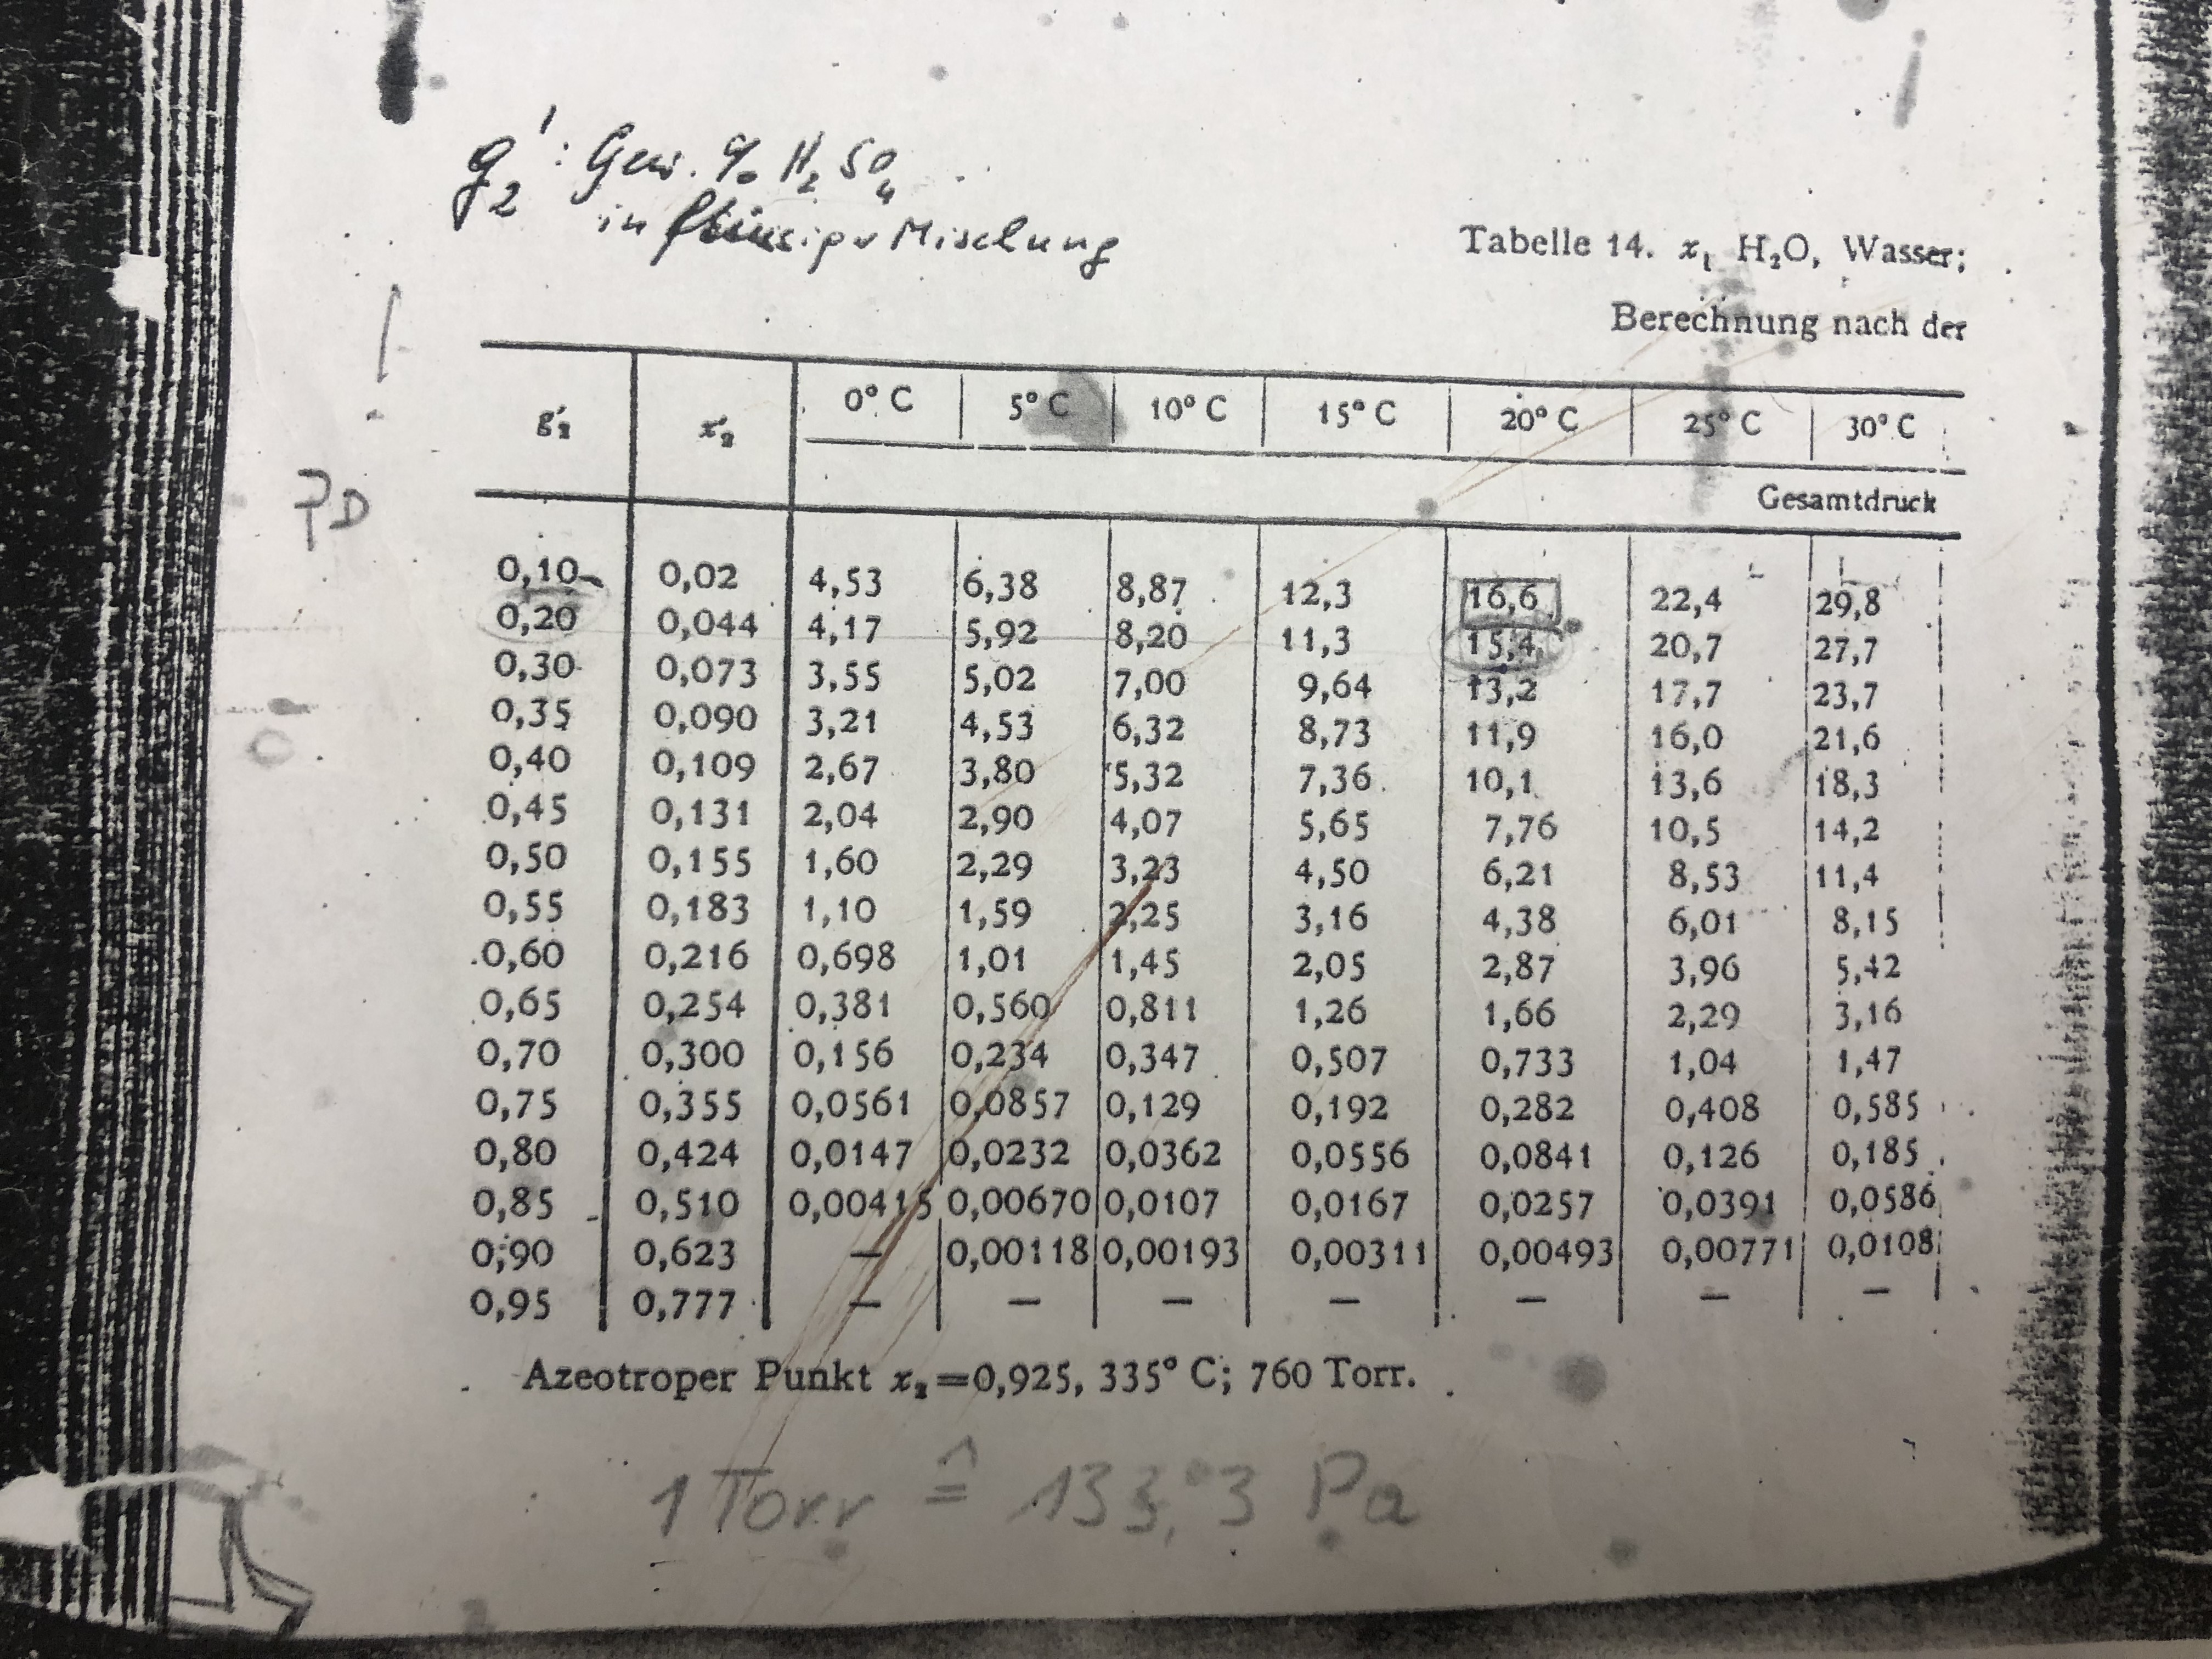
\includegraphics[width=0.7\textwidth]{tab}
	\end{center}
	\caption{vorliegende Tabelle 1}
	\label{fig:tab1}
\end{figure}

\begin{figure}[H]
	\begin{center}
		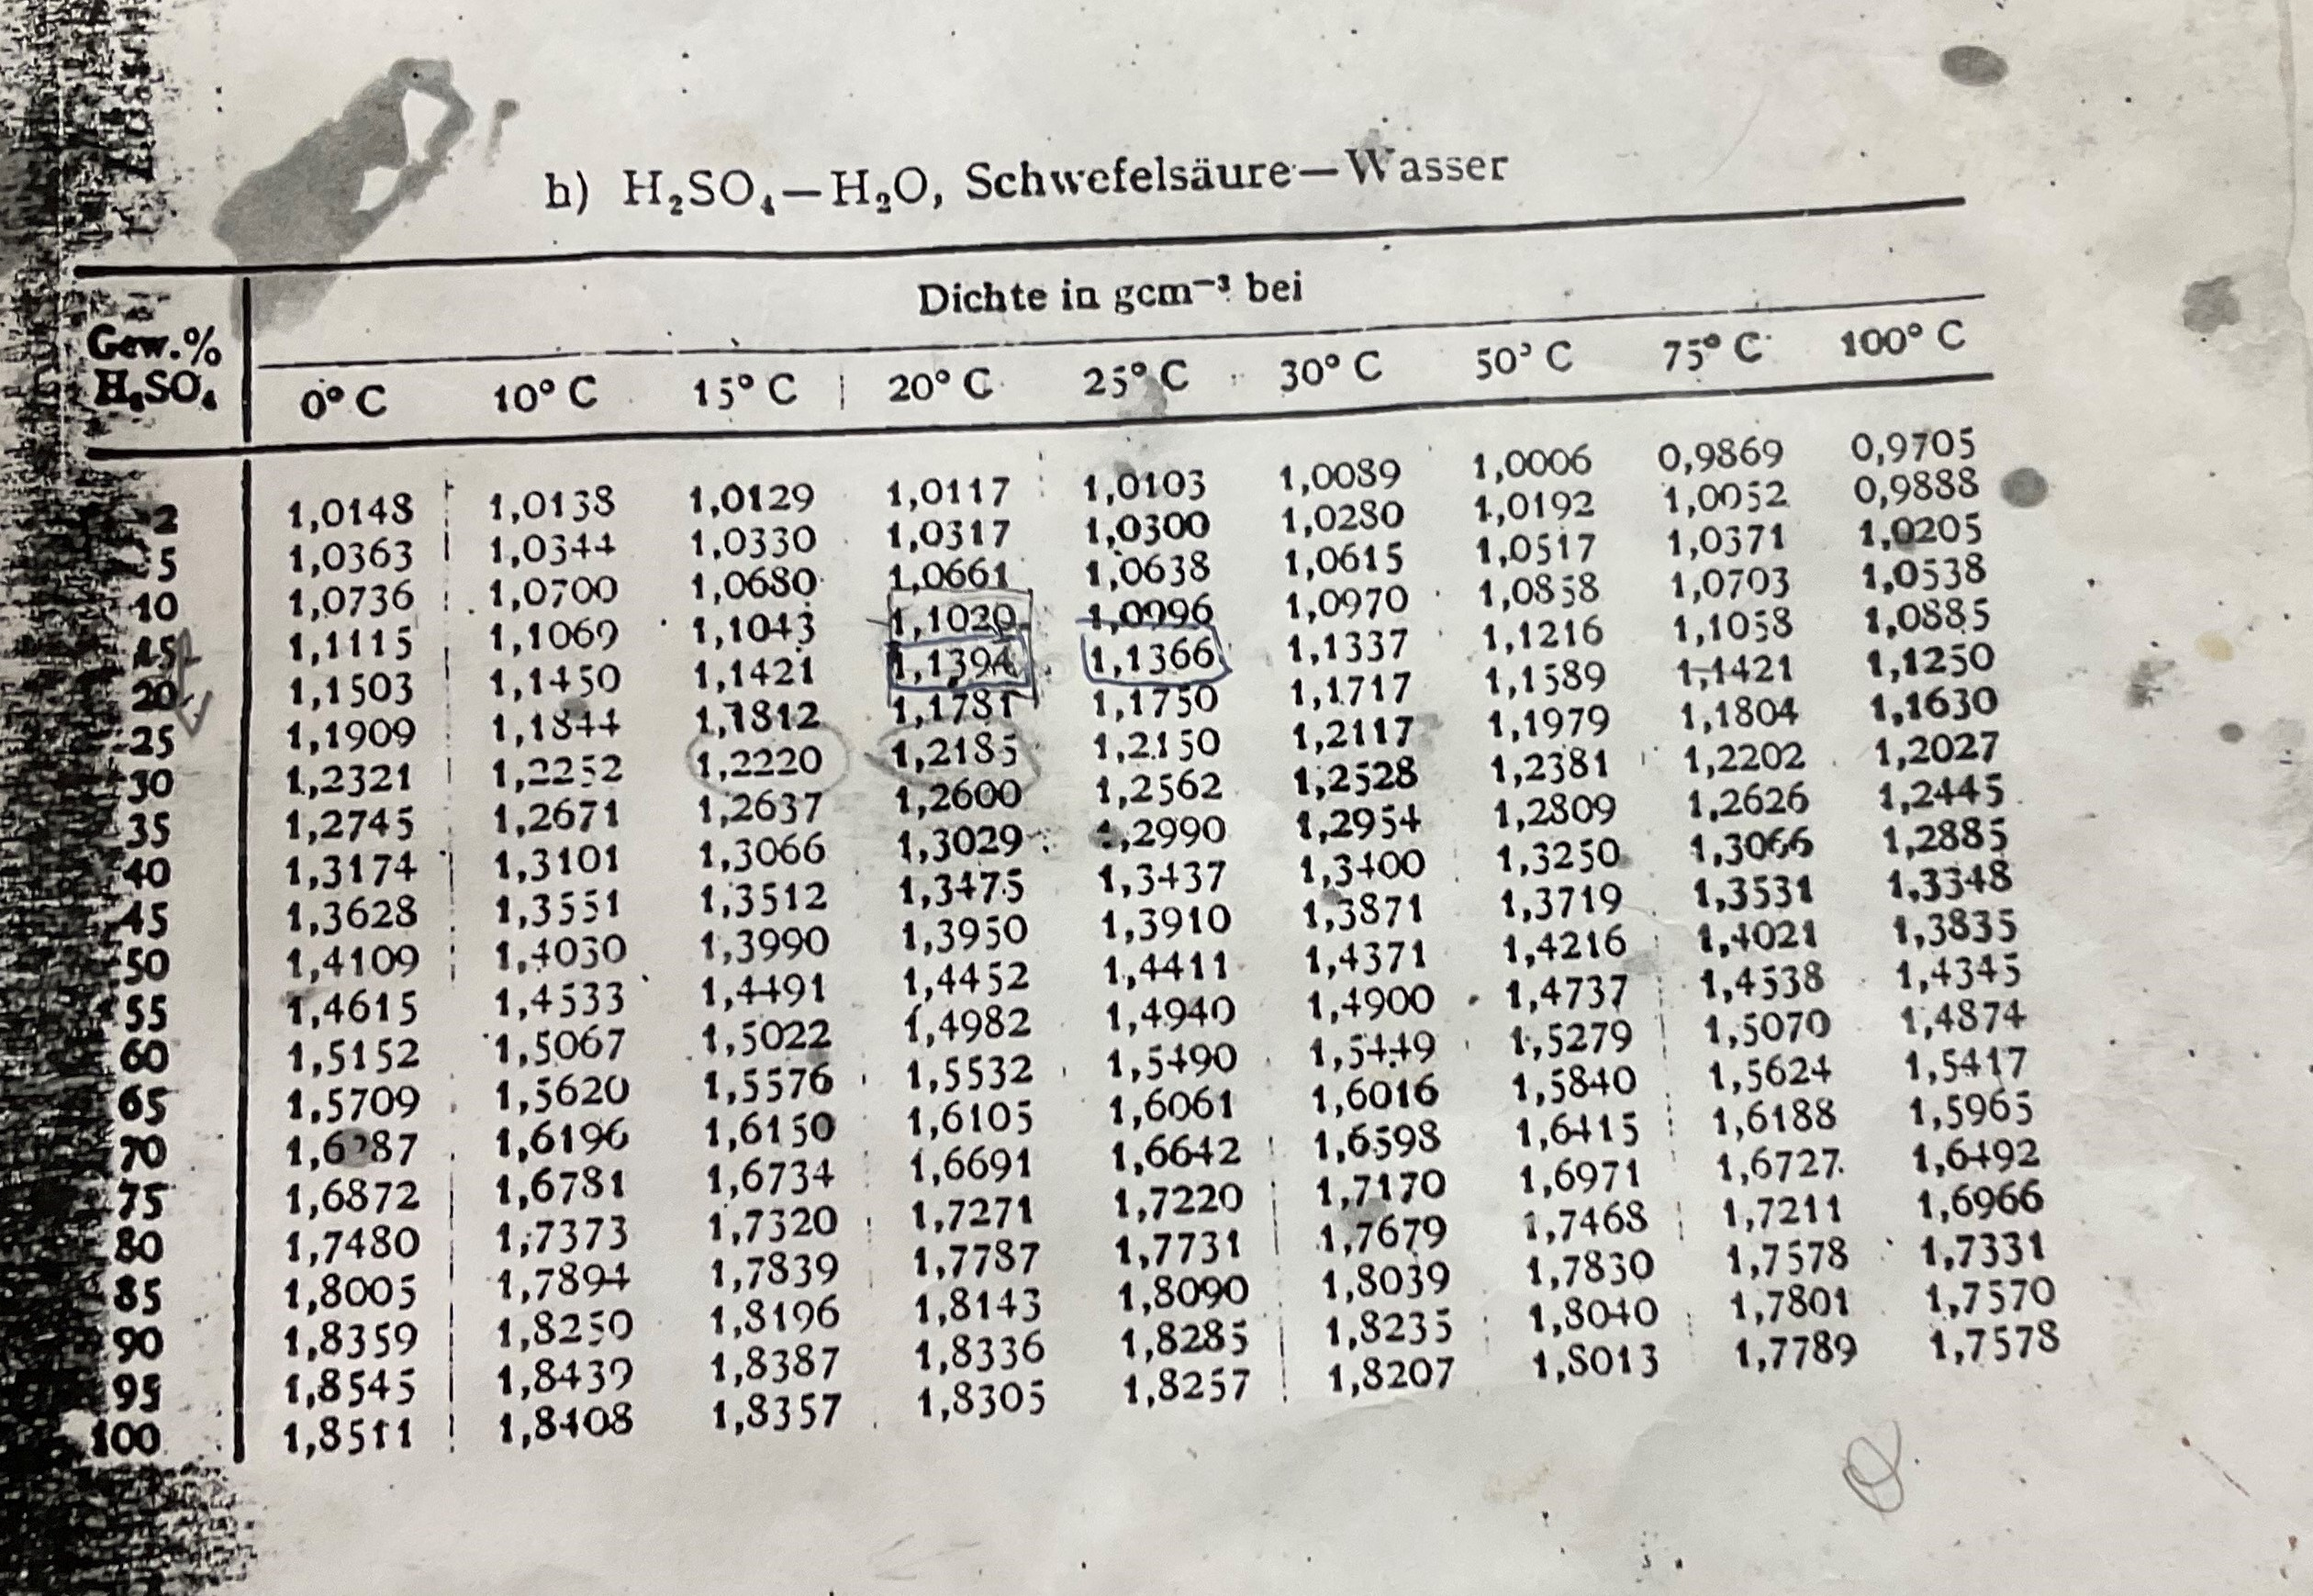
\includegraphics[width=0.7\textwidth]{tab_2}
	\end{center}
	\caption{vorliegende Tabelle 2}
	\label{fig:tab2}
\end{figure}

Daraus ergibt sich schließlich folgender Dampfdruck:

\begin{equation}
	\rho_D = \SI{18.1(11)}{\torr} = \SI{2400(140)}{\pascal}
	\label{eq:}
\end{equation}

Weiters müssen noch die Volumsdifferenzen aus den Werten von \autoref{tab:el_1}
und \autoref{tab:el_2} gebildet werden, wodurch folgende Werte entstehen:

\begin{table}[H]
	\caption{Volumsdifferenzen aus den Elektrolysen \\
		$L \dots$ linkes Rohr\\
		$R \dots$ rechtes Rohr\\
		$\Delta V_1 \dots$ erhaltene Volumsdifferenz bei Versuch 1\\
		$\Delta V_2 \dots$ erhaltene Volumsdifferenz bei Versuch 2}
	\label{tab:volumsdiff}
	\begin{center}
		\begin{tabular}[c]{r|S[table-format=2.2(2)]|S[table-format=2.2(2)]}
			\hline
			\multicolumn{1}{c|}{}                        &
			\multicolumn{1}{c|}{$\Delta V_1$ / \si{\ml}} &
			\multicolumn{1}{c}{$\Delta V_2$ / \si{\ml}}                      \\
			\hline
			L                                            & 24.7(4) & 29.2(4) \\
			R                                            & 12.0(4) & 14.8(4) \\
			\hline
		\end{tabular}
	\end{center}
\end{table}


Setzt man nun alle erhaltenen Werte in mit den zugehörigen Strömen und Zeiten in
\autoref{eq:Faraday_elektro} ein so erhält man schließlich folgende Werte für
die Faraday-Konstanten:

\begin{table}[H]
	\caption{erhaltene Werte für die Faradaykonstanten\\
		H$_2 \dots$ Wasserstoff\\
		O$_2 \dots$ Sauerstoff\\
		$F_1 \dots$ erhaltene Faraday-Konstante aus Versuch 1\\
		$F_2 \dots$ erhaltene Faraday-Konstante aus Versuch 2}
	\label{tab:}
	\begin{center}
		\begin{tabular}[c]{r|S[table-format=1.2(2)e3]|S[table-format=1.2(2)e3]}
			\hline
			\multicolumn{1}{c|}{\textbf{Gase}}                 &
			\multicolumn{1}{c|}{$F_1$ / \si{\coulomb\per\mol}} &
			\multicolumn{1}{c}{$F_2$ / \si{\coulomb\per\mol}}                            \\
			\hline
			{H$_2$}                                            & 9.3(3)e+04 & 9.5(3)e+04 \\
			{O$_2$}                                            & 9.7(4)e+04 & 9.4(4)e+04 \\
			\hline
		\end{tabular}
	\end{center}
\end{table}

Schließlich wird aus diesen vier Werte für die Faradaykonstante der Mittelwert gebildet, was folgenden Wert liefert. Für die Unsicherheit wurde dabei der Student t Faktor für ein 1-$\sigma$ und n=4 Messwerte berücksichtigt:

\begin{equation}
	F = \SI{9.47(7)e4}{\coulomb\per\mol}
	\label{eq:Fmittel}
\end{equation}

Unter Verwendung von
\autoref{eq:elektrochem} und dem zuvor ermittelten Mittelwert der Faradaykonstante aus \autoref{eq:Fmittel} kann mit
der molaren Masse von Sauerstoff ($M_{\text{H}}$, z=2) und Wasserstoff ($M_{\text{O}}$, z=1), die im folgenden ersichtlich sind, das entsprechende elektrochemische Äquivalent berechnet werden, was folgende Werte aus \autoref{tab:elektrochem} ergibt.

\begin{align*}
	M_{\text{H}} & = \SI{1.00784}{\g\per\mol}\cite{Kuchling} \\
	M_{\text{O}} & = \SI{15.999}{\g\per\mol}\cite{Kuchling}
\end{align*}

\begin{table}[H]
	\caption{bestimmte elektrochemische Äquivalente\\
		H$_2 \dots$ Wasserstoff\\
		O$_2 \dots$ Sauerstoff\\
		$C \dots$ bestimmtes elektrochemische Äquivalent}
	\label{tab:elektrochem}
	\begin{center}
		\begin{tabular}[c]{r|S[table-format=1.2(2)e3]}
			\hline
			\multicolumn{1}{c|}{\textbf{Gase}} &
			\multicolumn{1}{c}{$C$ / \si{\g\per\ampere\per\second}} \\
			\hline
			{H$_2$}                            & 1.07(2)e-05        \\
			{O$_2$}                            & 8.4(3)e-05         \\
			\hline
		\end{tabular}
	\end{center}
\end{table}

Unter Verwendung des zuvor bestimmten Mittelwerts für die Faraday Konstante lässt sich die Elementarladung nach folgender \autoref{eq:elementar_l_m_f} bestimmen.

\begin{equation}
	e = \frac{F}{N_A}
	\label{eq:elementar_l_m_f}
\end{equation}

Dies liefert schlussendlich folgenden Wert für die Elementarladung:

\begin{equation}
	e = \SI{1.57(4)e-19}{\ampere\second}
	\label{eq:elekto_elem}
\end{equation}

\newpage

\section{Diskussion}\label{disk}

\subsection{Silbercoulometer}

Da der Massendefekt durch Mechanischen Verarbeitungsschritte und dem Abbrechen
des Kristalls nicht genau bestimmt werden konnte, musste eine größere Unsicherheit
verwendet werden um die Elementarladung zu bestimmen, wodurch das Fehlerintervall, des Ergebnisses
größer wurde.

\vspace{2mm}

Die erhaltenen Ergebnisse sind im folgenden den entsprechenden Literaturwerten gegenübergestellt.

\begin{align*}
	F_{Literatur} & \approx \SI{9.65e4}{\coulomb\per\mol} \\
	F_{Anode}     & = \SI{10.6(11)e4}{\coulomb\per\mol}
\end{align*}

\begin{align*}
	e_{Literatur} & \approx \SI{1.602176634e-19}{\ampere\second} \\
	e_{Anode}     & = \SI{1.8(3)e-19}{\ampere\second}
\end{align*}

Betrachtet man die erhaltenen Werte wird deutlich, dass die Literaturwerte im Fehlerintervall enthalten sind, welches jedoch, wie bereits zuvor erwähnt, verkleinert werden hätte müssen, um bessere Aussagen anhand des Versuchs treffen zu können.

\vspace{2mm}

Weiters ist festzuhalten, dass die Silbernitratlösung mit Kupfernitrat verunreinigt war, was klar
an der Farbe der Flüssigkeit (bläulich) erkennbar war. Dies beeinträchtigt die Reaktion und somit
das Resultat dieses Experiments. Diese Verunreinigung lässt sich auf die Lötstelle bei den Anoden und Kathoden zurückführen.

\vspace{2mm}

Ein Verbesserungsvorschlag wäre statt Verlötungen diese Stellen eine Punktschweißung durchzuführen.

\vspace{2mm}

Weiters sollte der Massendefekt genauer bestimmt werden, indem der Niederschlag und die abgebrochenen Teile bei der Kathode berücksichtigt werden, indem das Gewicht des Gefäßes vor und nach der Messung bestimmt wird und so anhand der Gewichtszunahme die Masse der Niederschläge ermittelt werden kann. Auch hätte die Anode gründlicher abgebürstet werden sollen um auch die gelösten Rückstände die noch draufgeklebt sind, zu entfernen.

\newpage

\subsection{Elektrolyse}

Zunächst werden die erhaltenen Ergebnisse aus den Versuch den entsprechenden Literaturwerten gegenübergestellt.

\begin{align*}
	F_{\text{Literatur}} & = \SI{9.64853321233e4}{\coulomb\per\mol} \cite{SIstandard2019} \\
	F                    & = \SI{9.47(6)e4}{\coulomb\per\mol}
\end{align*}

\begin{align*}
	C_{\text{Wasserstoff,Literatur}} & = \SI{0,01044}{\mg\per\coulomb}\cite{Kuchling} \\
	C_{\text{Sauerstoff,Literatur}}  & = \SI{0,08291}{\mg\per\coulomb}\cite{Kuchling} \\
	C_{\text{Wasserstoff}}           & = \SI{1.07(2)e-02}{\mg\per\coulomb}            \\
	C_{\text{Sauerstoff}}            & = \SI{8.4(3)e-02}{\mg\per\coulomb}
\end{align*}

\begin{align*}
	e_{\text{Literatur}} & \approx \SI{1.602176634e-19}{\ampere\second}\cite{SIstandard2019} \\
	e                    & = \SI{1.57(4)e-19}{\ampere\second}
\end{align*}

Anhand der aufgelisteten Werte wird deutlich, dass die die Literaturwerte der elektrochemischen Äquivalente und der Elementarladung beinahe in den Fehlerintervallen der erhaltenen Werte enthalten sind. Der ermittelte Wert der Faraday-Konstanten liegt nur knapp nicht im Fehlerintervall. Allerdings ist dabei anzumerken, dass bei der Student t Verteilung nur von einem einfachen $\sigma$ Intervall bei der Berechnung des Mittelwerts der Faraday -Konstanten ausgegangen wurde.

\vspace{2mm}

Aufgrund \autoref{eq:Faraday_elektro} und aufgrund der verschiedenen Größenordnungen der einzelnen Therme, wird sichtbar, dass sich vor allem der Fehler des Volumens maßgeblich auf die Unsicherheit auswirkt und besonders der Fokus der Genauigkeit auf die Bestimmung dieses Werts gerichtet werden sollte.

Ein Verbesserungsvorschlag hierzu wäre, ein computerunterstütztes Messverfahren zu verwenden, um die genauen Volumina festzustellen, da das manuelle Ablesen der Werte von der Skala, besonders durch den leichten Kapillareffekt der Flüssigkeit in der Röhre, eine potentielle Fehlerquelle darstellt.

\newpage

\section{Zusammenfassung}

Im Folgenden sind die erhaltenen Ergebnisse nochmals aufgelistet:

\subsection{Silbercoulometer}

Für die Faraday - Konstante $F$ wurde anhand des Silbercoulometer folgender Wert bestimmt. Dabei ist anzumerken, dass hier nur der bestimmte Wert der Anode aufgelistet wird, da der entsprechende Wert der Kathode, aus bereits angesprochenen Gründen, nicht aussagekräftig ist.

\begin{align*}
	F = \SI{10.6(11)e4}{\coulomb\per\mol}
\end{align*}

Für die Elementarladung $e$, wurde anhand dieser Konstanten folgender Wert Berechnet:

\begin{align*}
	e = \SI{1.8(3)e-19}{\ampere\second}
\end{align*}

\subsection{Elektrolyse}

Zunächst wird die Dichte der H$_2$SO$_4$ Lösung bestimmt, was folgenden Wert liefert:

\begin{align*}
	\rho = \SI{1110(4)}{\g\per\L}
\end{align*}

Anhand der Elektrolysen wurde folgender Wert für die Faraday-Konstante bestimmt:

\begin{align*}
	F = \SI{9.47(6)e4}{\coulomb\per\mol}
\end{align*}

Für die elektrochemischen Äquivalente ergeben sich folgende Werte:

\begin{align*}
	C_{Wasserstoff} & = \SI{1.07(2)e-02}{\mg\per\coulomb} \\
	C_{Sauerstoff}  & = \SI{8.4(3)e-02}{\mg\per\coulomb}
\end{align*}

Für die Elementarladung $e$ ergibt sich folgender Wert:

\begin{align*}
	e & = \SI{1.57(4)e-19}{\ampere\second}
\end{align*}


\section{Anmerkungen}

Die ersten 3 Kapitel, sowie die dazugehörigen Abbildungen, wurden nicht von den
Autoren persönlich erstellt, sondern sind schon im Zuge der Aufgabenstellung,
in Form einer PDF, bereitgestellt und davon entnommen worden. \cite{vorlagesilber}


\newpage

\printbibliography
\listoffigures
\listoftables
\end{document}
